% siminos/presentations/Moscow20/Moscow20.tex
% $Author: predrag $ $Date: 2021-03-04 01:16:29 -0500 (Thu, 04 Mar 2021) $

%  started with ... presentations/Harvard19/Harvard19.tex   2019-03-31
%  started with siminos/presentations/GTMAP18/GTMAP18.tex   2018-04-13
%  started with siminos/presentations/GTmath18/GTmath18.tex 2018-02-24
%  started with siminos/presentations/KITP17/UCSB17.tex     2017-01-26
%  started with siminos/presentations/Israel16/Israel16.tex 2016-08-17
%  started with siminos/presentations/GTmap16/GTmap16.tex   2016-08-17
%  started with talks/predrag/NBI16/NBI16.tex               2016-04-25
%  started with talks/predrag/RoySoc16/RoySoc16.tex         2016-04-25

\input ../../inputs/layoutBeamer
\usepackage[font=scriptsize, labelfont=bf]{caption}
\usepackage[
    backend=biber,  %bibtex,
    sorting=nyt,
    %refsection=chapter,
    %citereset=chapter,
    style=numeric, %alphabetic, % %style=authoryear,
    natbib=true,
    style=phys, % aps
    biblabel= brackets, % superscript, %
    articletitle=false, % true,  % false, % aps
    %chaptertitle=true,  % aip;  % false, % aps
    pageranges = true , % aip: the full range
             % = false, % aps: only the first page being printed
    sortlocale=en_US,
    firstinits=true,
    url=false, %true,  %
    doi=false, %true,
    eprint=false
]{biblatex}
\addbibresource{../../bibtex/siminos.bib}
\setbeamerfont{footnote}{size=\tiny}
% dasbuch/book/inputs/def.tex
% $Author: predrag $ $Date: 2021-07-23 16:15:21 -0400 (Fri, 23 Jul 2021) $

%%%%%%%%%%%%%%%%%%%%%%%%%%%%%%%%%%%%%%%%%%%%%%%%%%%%%%%%%%%%%%%%%%%%%%%%%
%% defines macros used throughout ChaosBook and related
%%%%%%%%%%%%%%%%%%%%%%%%%%%%%%%%%%%%%%%%%%%%%%%%%%%%%%%%%%%%%%%%%%%%%%%%%

%               Predrag         17dec2020
%               Predrag         23may2020
%               Predrag          6oct2017
% \input{inputs/defBtracks} after def.tex to pdfLaTeX birdtracks macros
%               Predrag         11apr2015
% collected group theoretic macros
%               Predrag         25jan2014
% defined graphicspath
%               Predrag         15sep2013
% \goodbreak arXiv -> arXiv
%               Predrag         27feb2012
%               Predrag         17feb2012
%               Predrag          4feb2012
%               Predrag          9oct2009
%               Predrag         12jun2008
%               Predrag         15dec2008
%               Predrag         29oct2005
%               Predrag         13jul2005
%               Predrag         24apr2005
%               Predrag         14feb2005
%               Predrag         22jan2005
%               Predrag         16nov2004
%               Predrag         13jun2004
%               Predrag          3may2004
%               Predrag         10apr2004
%               Predrag         21feb2004
%               Predrag          4oct2003
%               Predrag         30aug2003
%               Predrag         20jun2003
%               Predrag         17jan2003
%               Predrag          6dec2002
%               Predrag          7jul2002
%               Predrag         19nov2000
%               Ronnie          23sep2000
% Predrag disabled \basedirectory machine identifier    25aug2000
% Predrag created               30oct1994

    %%%%%%% CL18 specific %%%%%%%%%%%%%%%%%%%%%%%%%%%%
\newcommand{\fundPip}{fundamental parallelepiped}
\newcommand{\brick}{block}
\newcommand{\Brick}{Block}
\newcommand{\jacobianOrb}{orbit Jacobian matrix}
\newcommand{\JacobianOrb}{Orbit Jacobian matrix}
\newcommand{\jacobianOrbs}{orbit Jacobian matrices}
\newcommand{\JacobianOrbs}{Orbit Jacobian matrices}
\newcommand{\HillDet}{Hill determinant}
\newcommand{\PV}{Percival-Vivaldi}
\newcommand{\AW}{Adler-Weiss}
% \newcommand{\GO}{Gutkin-Osipov}
\newcommand{\SLn}[2]{\ensuremath{\textrm{SL}_{#1}(#2)}}
\newcommand{\jMorb}{{\ensuremath{\cal \jMps}}}
\newcommand{\conf}{\ensuremath{x}}      % Configuration space coordinate
\newcommand{\lattice}{\ensuremath{\mathcal{L}}}
\newcommand{\jMat}{\mathbb{\jMps}}

    %%%%%% Boris definitions  %%%%%%%%%%%%%%%%%%%%%%%%%%%%
\newcommand{\Aa}{\ensuremath{\bar{\A}}}         % alphabet with a bar
\newcommand{\A}{\ensuremath{\mathcal{A}}}       % alphabet
% \newcommand{\Ai}{\ensuremath{\mathcal{A}_0}}    % alphabet inner
% \newcommand{\Ae}{\ensuremath{\mathcal{A}_1}}    % alphabet outer
% \newcommand{\R}{\ensuremath{\mathcal{R}}}
% \newcommand{\m}{\ensuremath{\mathsf{m}}}     % Boris
% \newcommand{\m}{\ensuremath{m}}     % Predrag experimental 2016-11-08
\newcommand{\Mm}{\ensuremath{\mathsf{M}}}
% \newcommand{\MmR}{\Mm_\R}
\newcommand{\Xx}{\ensuremath{\mathsf{X}}}
% \newcommand{\Zz}{\ensuremath{\mathbb{Z}^2}}
% \newcommand{\Spshift}{\mathrm{S}}
% \newcommand{\Tshift}{\mathrm{T}}
% \newcommand{\Pol}{\mathcal{P}}                  % Boris
% \newcommand{\ZLT}{\mathbb{Z}^2_{\scriptscriptstyle\mathrm{LT}}}
%\newcommand{\q}{\ensuremath{\mathsf{m}}}     % Boris
% \newcommand{\q}{\ensuremath{q}}     % Predrag experimental 2016-11-08
% \newcommand{\D}{\mathcal{D}}
% \newcommand{\gd}{\mathsf{g}}
% \newcommand{\gp}{\mathsf{g}^0}


\ifpaper % prepare for B&W paper printing:
       \newcommand{\href}[2]{{#2}}  % no hyperref
       \newcommand{\HREF}[2]{{#2}}
       \renewcommand{\color}[1]{}       % B&W
       \newcommand{\wwwcb}[1]{{ChaosBook.org#1}}
       \newcommand{\wwwgt}{{birdtracks.eu}}
       \newcommand{\wwwQFT}[1]{{ChaosBook.org/\-Field\-Theory#1}}
       \newcommand{\wwwcnsQFT}[1]{{ChaosBook.org/\-Field\-Theory#1}}
       \newcommand{\weblink}[1]{{#1}}
       \newcommand{\arXiv}[1]{{arXiv:#1}}
       \newcommand{\bioRxiv}[1]{{bioRxiv:#1}}
       \newcommand{\mpArc}[1]{{mp\_arc~#1}}
\else % prepare hyperlinked pdf
        \newcommand{\wwwcb}[1]{       % keep homepage flexible:
                  {\href{http://ChaosBook.org#1}
              {ChaosBook.org#1}}}
       \newcommand{\wwwgt}{{\href{http://birdtracks.eu}
              {birdtracks.eu}}}
       \newcommand{\wwwQFT}[1]{
                  {\href{http://ChaosBook.org/FieldTheory#1}
              {ChaosBook.org/\-Field\-Theory#1}}}
       \newcommand{\wwwcnsQFT}[1]{
                  {\href{http://ChaosBook.org/FieldTheory#1}
              {ChaosBook.org/\-Field\-Theory#1}}}
       \newcommand{\weblink}[1]{{\href{http://#1}{#1}}}
       \newcommand{\HREF}[2]{
              {\href{#1}{#2}}}
       \newcommand{\mpArc}[1]{
              {\href{http://www.ma.utexas.edu/mp_arc-bin/mpa?yn=#1}
                   {mp\_arc~#1}}}
       \newcommand{\arXiv}[1]{
              {\href{https://arXiv.org/abs/#1}{arXiv:#1}}}
       \newcommand{\bioRxiv}[1]{
              {\href{https://biorxiv.org/content/10.1101/#1}{bioRxiv:#1}}}
\fi

%%%%%%%%%%%%%%%%%%%%%% QUOTATIONS %%%%%%%%%%%%%%%%%%%%%%%%%%%%%%%%%%%%%%
%
%  the learned/witty quotes at the chapter and section headings
%
\newsavebox{\bartName}
\newcommand{\bauthor}[1]{\sbox{\bartName}{\parbox{\textwidth}{\vspace*{0.8ex}
       %\hspace*{\fill}
       \hspace{2em}---\small\noindent #1}}}
\newenvironment{bartlett}{\hfill\begin{minipage}[t]{0.65\textwidth}\small}%
{\hspace*{\fill}\nolinebreak[1]\usebox{\bartName}\vspace*{1ex}\end{minipage}}
%
%  a quotation inserted into the text
%
\newenvironment{txtquote}{\begin{quotation} \small}{\end{quotation}}

\newcommand{\student}{Henriette Roux}
%\newcommand{\student}{Jens J. Jensen}

%%%%%%%%%%%%%%%%%%%%%% INDEXING %%%%%%%%%%%%%%%%%%%%%%%%%%%%%%%%%%%%%%%%%
\newcommand{\indx}[1] {#1\index{#1}}    % do not need to repeat the word

\newcommand{\file}[1]{$\footnotemark\footnotetext{{\bf file} #1}$}
% PC 9sep2008 commented out (is it used?):
%\newcommand{\lecture}[2]{ \addtocontents{toc}
%           {{\scriptsize #1}{\sf\small lecture: \scriptsize #2}} }

%%%%%%%%%%%%%%% EQUATIONS %%%%%%%%%%%%%%%%%%%%%%%%%%%%%%%
\newcommand{\beq}{\begin{equation}}
\newcommand{\continue}{\nonumber \\ }
\newcommand{\nnu}{\nonumber}
\newcommand{\eeq}{\end{equation}}
\newcommand{\ee}[1] {\label{#1} \end{equation}}
\newcommand{\bea}{\begin{eqnarray}}
\newcommand{\ceq}{\nonumber \\ & & }
\newcommand{\eea}{\end{eqnarray}}
\newcommand{\barr}{\begin{array}}
\newcommand{\earr}{\end{array}}

%%%%%%%%%%%%%%% REFERENCING EQUATIONS ETC. %%%%%%%%%%%%%%%%%%%%%%%%%%%%%%%
\newcommand{\rf}     [1] {~\cite{#1}}
\newcommand{\refref} [1] {ref.~\cite{#1}}
\newcommand{\refRef} [1] {Ref.~\cite{#1}}
\newcommand{\refrefs}[1] {refs.~\cite{#1}}
\newcommand{\refRefs}[1] {Refs.~\cite{#1}}
\newcommand{\refeq}  [1] {(\ref{#1})}
            % in amstex, \eqref is predefined and better than \refeq
\newcommand{\refeqs} [2]{(\ref{#1}--\ref{#2})}
\newcommand{\refpage}[1] {page~\pageref{#1}}
\newcommand{\reffig} [1] {figure~\ref{#1}}
\newcommand{\reffigs} [2] {figures~\ref{#1} and~\ref{#2}}
\newcommand{\refFig} [1] {Figure~\ref{#1}}
\newcommand{\refFigs} [2] {Figures~\ref{#1} and~\ref{#2}}
\newcommand{\reftab} [1] {table~\ref{#1}}
\newcommand{\refTab} [1] {Table~\ref{#1}}
\newcommand{\reftabs}[2] {tables~\ref{#1} and~\ref{#2}}
\newcommand{\refsect}[1] {sect.~\ref{#1}}
\newcommand{\refsects}[2] {sects.~\ref{#1} and \ref{#2}}
\newcommand{\refSect}[1] {Sect.~\ref{#1}}
\newcommand{\refSects}[2] {Sects.~\ref{#1} and \ref{#2}}
\newcommand{\refsecttosect}[2] {Sects.~\ref{#1} to~\ref{#2}}
\newcommand{\refchap}[1] {chapter~\ref{#1}}
\newcommand{\refChap}[1] {Chapter~\ref{#1}}
\newcommand{\refchaps}[2] {chapters~\ref{#1} and~\ref{#2}}
\newcommand{\refchaptochap}[2] {chapters~\ref{#1} to~\ref{#2}}
\newcommand{\refappe}[1] {appendix~\ref{#1}}
\newcommand{\refappes}[2] {appendices~\ref{#1} and~\ref{#2}}
\newcommand{\refAppe}[1] {Appendix~\ref{#1}}
\newcommand{\refrem} [1] {remark~\ref{#1}}
\newcommand{\refRem} [1] {Remark~\ref{#1}}
\newcommand{\refexam}[1] {example~\ref{#1}}
\newcommand{\refExam}[1] {Example~\ref{#1}}
\newcommand{\refexer}[1] {exercise~\ref{#1}}
\newcommand{\refExer}[1] {Exercise~\ref{#1}}
\newcommand{\refsolu}[1] {solution~\ref{#1}}
\newcommand{\refSolu}[1] {Solution~\ref{#1}}

%%%%%%%%%%%%%%  Abbreviations %%%%%%%%%%%%%%%%%%%%%%%%%%%%%%%%%%%%%%%%
%%% APS (American Physiology Society, it seems) style:
%%%     Latin or foreign words or phrases should be roman, not italic.
%%%     Insert a `hard' space after full points
%%%                                         that do not end sentences.

\newcommand{\etc}{{etc.}}       % APS
\newcommand{\etal}{{\em et al.}}    % etal in italics, APS too
\newcommand{\ie}{{i.e.}}        % APS
\newcommand{\cf}{{\em cf.\ }}     % APS
\newcommand{\eg}{{e.g.\ }}        % APS, OUP, hard space '\eg\ NextWord'
% \newcommand{\etc}{{\em etc.}}     % etcetera in italics
% \newcommand{\ie}{{that is}}       % use Latin or English?  Decide later.
% \newcommand{\cf}{{cf.}}
% \newcommand{\eg}{{\it e.g.,\ }}   % Wirzba 2sep2001

%%%%%%%%%%%%%%% ChaosBook Abbreviations %%%%%%%%%%%%%%%%%%%%%%%%

\newcommand{\evOper}{evolution oper\-ator}
\newcommand{\EvOper}{Evolution oper\-ator}
 %% \newcommand{\evOp}{Ruelle operator} %could be ``evolution'' instead?
%\newcommand{\FPoper}{Frobenius-Perron oper\-ator}
\newcommand{\FPoper}{Perron-Frobenius oper\-ator} % Pesin's ordering
\newcommand{\FP}{Perron-Frobenius}
\newcommand{\statesp}{state space}
\newcommand{\Statesp}{State space}
\newcommand{\stateDsp}{state-space}
\newcommand{\StateDsp}{State-space}
\newcommand{\fixedpnt}{fixed point}
\newcommand{\Fixedpnt}{fixed point}
\newcommand{\maslov}{topological}
\newcommand{\Maslov}{Topological}
%\newcommand{\Maslov}{Keller-Maslov}
\newcommand{\jacobian}{Jacobian}        % determinant
% \newcommand{\jacobianM}{fundamental matrix} % no known standard name?
% \newcommand{\jacobianMs}{fundamental matrices}  %
% \newcommand{\JacobianM}{Fundamental matrix} %
% \newcommand{\JacobianMs}{Fundamental matrices}  %
\newcommand{\jacobianM}{Jacobian matrix}  % back to Predrag's name 20oct2009
\newcommand{\jacobianMs}{Jacobian matrices}   % matrices
\newcommand{\JacobianM}{Jacobian matrix} %
\newcommand{\JacobianMs}{Jacobian matrices}  %
\newcommand{\FloquetM}{Floquet matrix} % specialized to periodic orb
\newcommand{\FloquetMs}{Floquet matrices}  %
% \newcommand{\stabmat}{matrix of variations}   % Arnold, says Vattay
\newcommand{\stabmat}{stability matrix}     % stability matrix, velocity gradients
\newcommand{\Stabmat}{Stability matrix}     % Stability matrix
\newcommand{\stabmats}{stability matrices}
\newcommand{\monodromyM}{monodromy matrix} % monodromy matrix, Poincare cut
\newcommand{\MonodromyM}{Monodromy matrix} % monodromy matrix, Poincare cut
\newcommand{\dzeta}{dyn\-am\-ic\-al zeta func\-tion}
\newcommand{\Dzeta}{Dyn\-am\-ic\-al zeta func\-tion}
\newcommand{\tzeta}{top\-o\-lo\-gi\-cal zeta func\-tion}
\newcommand{\Tzeta}{Top\-o\-lo\-gi\-cal zeta func\-tion}
\newcommand{\BERzeta}{BER zeta func\-tion}
%\newcommand{\tzeta}{Artin-Mazur zeta func\-tion} %alternative to topological
\newcommand{\qS}{semi\-classical zeta func\-tion}
%\newcommand{\qS}{Gutz\-willer-Voros zeta func\-tion}
\newcommand{\Gt}{Gutz\-willer trace formula}
\newcommand{\Fd}{spec\-tral det\-er\-min\-ant}
%\newcommand{\fd}{spec\-tral det\-er\-min\-ant} %in many articles
\newcommand{\FD}{Spec\-tral det\-er\-min\-ant}
\newcommand{\cFd}{semiclass\-ic\-al spec\-tral det\-er\-mi\-nant}
\newcommand{\cFD}{Semiclass\-ic\-al spec\-tral det\-er\-mi\-nant}
% \newcommand{\cFd}{semiclass\-ic\-al Fred\-holm det\-er\-mi\-nant}
\newcommand{\Vd}{Vattay det\-er\-mi\-nant}
\newcommand{\cycForm}{cycle averaging formula}
\newcommand{\CycForm}{Cycle averaging formula}
\newcommand{\freeFlight}{mean free flight time}
\newcommand{\FreeFlight}{Mean free flight time}
\newcommand{\pdes}{partial differential equations}
\newcommand{\Pdes}{Partial differential equations}
% \newcommand{\dof}{dof}         % Hamiltonian deegree of freedom
\newcommand{\dof}{degree of freedom}
% \newcommand{\Dof}{Degree of freedom}
\newcommand{\dofs}{degrees of freedom}
% \newcommand{\Dofs}{Degrees of freedom}
\newcommand{\cdof}{computational degree of freedom}
\newcommand{\Cdof}{Computational degree of freedom}
\newcommand{\cdofs}{computational degrees of freedom}
\newcommand{\Cdofs}{Computational degrees of freedom}

%%%%%%%%%%%%%%% VECTORS, MATRICES, NORMS %%%%%%%%%%%%%%%%%%%%%%%%%%%%%%%%%

	% without large brackets:
\newcommand{\braket}[2]
		   {\langle{#1}\vphantom{#2}|\vphantom{#1}{#2}\rangle}
\newcommand{\bra}[1]{\langle{#1}\vphantom{ }|}
\newcommand{\ket}[1]{|\vphantom{}{#1}\rangle}
	% with large brackets:
%\newcommand{\bra}[1]{\left\langle{#1}\vphantom{ }\right|}
%\newcommand{\ket}[1]{\left|\vphantom{}{#1}\right\rangle}
%\newcommand{\braket}[2]{\left\langle{#1}
%                        \vphantom{#2}\right|\left.\vphantom{#1}
%                        {#2}\right\rangle}

\newcommand{\dual}[1]{{#1}^\dag}
% \newcommand{\dual}[1]{{#1}^\ast}
% \newcommand{\transp}[1]{\bar{#1}}
% \newcommand{\transp}[1]{{#1}{}^T}
\newcommand{\transp}[1]{{#1}{}^\top}

% Commented out AMS-style pmatrix, which is incompatible with TeX/LaTeX pmatrix
% used throughout dasbuch. Fri Oct 12 15:51:03 EDT 2007

\newcommand{\MatrixII}[4]{\left[
\begin{array}{cc}
{#1}  &  {#2} \\
{#3}  &  {#4} \end{array} \right]}
% a problem with \pmatrix 12oct 2007
%\newcommand{\MatrixII}[4]{
%   \begin{bmatrix}{#1}  &  {#2} \\
%                  {#3}  &  {#4} \end{bmatrix}}

\newcommand{\MatrixIII}[9]{
\begin{bmatrix}
  {#1}  &  {#2} &  {#3} \\
  {#4}  &  {#5} &  {#6} \\
  {#7}  &  {#8} &  {#9}
\end{bmatrix}
          }

\newcommand{\transpVectorII}[2]{
    \begin{bmatrix}{#1}  &  {#2}  \end{bmatrix}}

%\newcommand{\VectorII}[2]{\left(
%\begin{array}{cc}
%{#1}  &  {#2} \end{array} \right)}
%
%\newcommand{\VectorII}[2]{
%  \pmatrix{ {#1} \cr {#2}}
%}

 \newcommand{\VectorII}[2]{
    \begin{bmatrix} {#1} \\
                    {#2}  \end{bmatrix}}

 \newcommand{\VectorIII}[3]{
    \begin{bmatrix} {#1} \\
                    {#2} \\
                    {#3} \end{bmatrix}}

%\newcommand{\transpVectorII}[2]{\left(
%\begin{array}{c}
%   {#1} \cr
%   {#2}\end{array} \right)
%}

%\newcommand{\VectorIII}[3]{
%  \pmatrix{ {#1} \cr
%            {#2} \cr
%            {#3}
%          }
%}

\newcommand{\combinatorial}[2]{ {#1 \choose #2}}

%%%%%%%%%%%%%%% Sundry symbols within math eviron.: %%%%%%%%%%%%

\newcommand{\obser}{\ensuremath{a}}     % an observable from phase space to R^n
\newcommand{\Obser}{\ensuremath{A}}     % time integral of an observable
\newcommand{\onefun}{\iota} % the function that returns one no matter what
\newcommand{\defeq}{=}      % the different equal for a definition
\newcommand {\deff}{\stackrel{\rm def}{=}}
\newcommand{\reals}{\mathbb{R}}
\newcommand{\complex}{\mathbb{C}}
\newcommand{\integers}{\mathbb{Z}}
\newcommand{\rationals}{\mathbb{Q}}
\newcommand{\naturals}{\mathbb{N}}
\newcommand{\LieD}{{\mathcal{L}\!\!\llap{-}\,\,}}  % {{\pound}} % Lie Derivative
\newcommand{\half}{{\scriptstyle{\frac{1}{2}}}}
\newcommand{\pde}{\partial}
\newcommand{\pdfrac}[2]{\frac{\partial #1}{\partial #2}}
\renewcommand\Im{\ensuremath{\mathrm{Im}\,}}
\renewcommand\Re{\ensuremath{\mathrm{Re}\,}}
\renewcommand{\det}{\mathrm{det}\,}
\newcommand{\Det}{\mathrm{Det}\,}
\newcommand{\tr}{\mathrm{tr}\,}
\newcommand{\Tr}{\mathrm{Tr}\,}
\newcommand{\trDiscr}[2]{\Cn{#1}^{#2}}  % Xiong Ding
\newcommand{\sign}[1]{\sigma_{#1}}
%\newcommand{\sign}[1]{{\rm sign}(#1)}
\newcommand{\mInv}{{I}}                 % material invariant
\newcommand{\msr}{\ensuremath{\rho}}                % measure
\newcommand{\Msr}{{\mu}}                % coarse measure
\newcommand{\dMsr}{{d\mu}}              % measure infinitesimal
\newcommand{\SRB}{{\rho_0}}             % natural measure
\newcommand{\vol}{{V}}                  % volume of i-th tile
\newcommand{\prpgtr}[1]{\delta\negthinspace\left( {#1} \right)}
%\newcommand{\Zqm}{\ensuremath{Z_{qm}}}         % Gutz-Voros zeta function
\newcommand{\Zqm}{\ensuremath{\det(\hat{H} - E)_{sc} }} % semicls spectr. det:
\newcommand{\Fqm}{\ensuremath{F_{qm}}}
\newcommand{\zfct}[1]{\zeta ^{-1}_{#1}}
\newcommand{\zetaInv}{\ensuremath{1/\zeta}}
% \newcommand{\zetaInv}{{\zeta^{-1}}}
\newcommand{\zetatop}{\ensuremath{1/\zeta_{\mbox{\footnotesize top}} }}
\newcommand{\zetaInvBER}[1]{1/\zeta_{\mbox{\footnotesize BER}}(#1)}
\newcommand{\BER}[1]{{\mbox{\footnotesize BER}}} % Baladi-Ruelle-Eckmann
\newcommand{\eigCond}{\ensuremath{F}}           % eigenvalue cond. function
\newcommand{\expct}    [1]{\langle {#1} \rangle}
\newcommand{\spaceAver}[1]{\langle {#1} \rangle}
%\newcommand{\expct}    [1]{\left\langle {#1} \right\rangle}
%\newcommand{\spaceAver}[1]{\left\langle {#1} \right\rangle}
\newcommand{\timeAver} [1]{\overline{#1}}
\newcommand{\norm}[1]{\left\Arrowvert \, #1 \, \right\Arrowvert}
\newcommand{\pS}{\ensuremath{\mathcal{M}}}          % symbol for state space
\newcommand{\ssp}{\ensuremath{x}}                % state space point
\newcommand{\cssp}{\ensuremath{\tilde{u}}}                % Complex state space point
\newcommand{\csspR}{\ensuremath{b}}                % Real part of complex state space point
\newcommand{\csspI}{\ensuremath{c}}                % Imaginary part of complex state space point
\newcommand{\tissp}{\tilde{\Delta\ssp}} % Rytis \CostFct
\newcommand{\pSpace}{x}       % Hamiltonian phase space x=(q,p) coordinate
\newcommand{\coord}{q}        % configuration space p coordinate
\newcommand{\DOF}{\ensuremath{D}}          % Hamiltonian deegree of freedom
\newcommand{\NWS}{\ensuremath{\Omega}}     % symbol for the non--wandering set
\newcommand{\AdmItnr}{\Sigma}      % set of admissible itineraries
\newcommand{\intM}[1]{{\int_\pS{\!d #1}\:}} %state space integral
\newcommand{\Cint}[1]{\oint\frac{d#1}{2 \pi i}\;} %Cauchy contour integral
\newcommand{\Lint}[1]{\frac{1}{L}\!\oint d#1\,}
\newcommand{\PoincS}{\ensuremath{\mathcal{P}}}  % symbol for Poincare section
%\newcommand{\PoincS}{\partial\mathcal{M}}    % billiard Poincare section
\newcommand{\PoincM}{\ensuremath{P}}       % symbol for Poincare map
\newcommand{\PoincC}{\ensuremath{U}}       % symbol for Poincare constraint function
\newcommand{\arc}{\ensuremath{s}}          % symbol for billiard wall arc
\newcommand{\mompar}{\ensuremath{p}}       % billiard wall parall. momentum
%\newcommand{\mompar}{\ensuremath{p_\para}} % billiard wall parall. momentum
\newcommand{\restCoeff}{\ensuremath{\gamma}}  % billiard wall restitution coeff
\newcommand{\timeIn}[1]{{t^{-}_{#1}}}      % billiard wall time of arrival
\newcommand{\timeOut}[1]{{t^{+}_{#1}}}     % billiard wall time of departure
\newcommand{\Lop}{\ensuremath{\mathcal{L}}}       % evolution operator
\newcommand{\Uop}{\ensuremath{\mathcal{K}}}       % Koopman operator, Driebe notation
%\newcommand{\Uop}{\ensuremath{\mathcal{L}^\dagger}}  % Koopman, adjoint notation
\newcommand{\Aop}{\ensuremath{\mathcal{A}}}        % evolution generator
\newcommand{\TrOp}{\ensuremath{\mathcal{T}}}       % transfer operator, like in statmech

\newcommand{\matId}{\ensuremath{{\bf 1}}}       % matrix identity
\newcommand {\id}{{\ \hbox{{\rm 1}\kern-.62em\hbox{\rm 1}}}} % Roberto
\newcommand{\unit}{{\bf 1}}                     %% in lattFT.tex %%
                                                %experiment with {\bf 1\!\!\!1}
\newcommand{\Bell}{{\boldsymbol{\ell}}}
\newcommand{\eigenvL}{\ensuremath{s}}      % evolution operator eigenvalue
\newcommand{\inFix}[1]{{\in \mbox{\footnotesize Fix}f^{#1}}}
\newcommand{\inZero}[1]{{\in \mbox{\footnotesize Zero} \, f^{#1} }}
\newcommand{\xzero}[1]{{x_{#1}^\ast}}
\newcommand{\fractal}{{\mathcal{F}}}
\newcommand{\contract}{F}
% \newcommand{\presentation}{P} % PC commented out 7sep2008
\newcommand{\orderof}[1]{o(#1)} % Rytis 22mar2005

     %%%%%%%%%% flows: %%%%%%%%%%%%%%%%%%%%%%%%%%%%
\newcommand\map{f}                  % other people like \phi's etc
\newcommand\flow[2]{{f^{#1}(#2)}}
\newcommand{\vel}{\ensuremath{v}}   % state space velocity
\newcommand\velField[1]{{v(#1)}}    % ODE velocity field
\newcommand\invFlow{F}
\newcommand\hflow[2]{{\hat{f}^{#1}(#2)}}
\newcommand\timeflow{{f^\zeit}}
\newcommand\tflow[2]{{\tilde{f}^{#1}(#2)}}
%\newcommand\tflow{\tilde{f}^\tau}        %RECHECK USE OF THIS!
\newcommand\xInit{{\ssp_0}}        %initial x
%\newcommand\xInit{\xi}     %initial x, Spiegel notation
\newcommand{\para}{\parallel}
\newcommand\multiX{x}       %multi point n-dim vector
\newcommand\multiF{f}       %multi point n-dim vector mapping

   %%%%%%% 3D physical flow
\newcommand{\stagp}{stagnation point}
\newcommand{\Stagp}{Stagnation point}
\newcommand{\relstagp}{traveling stagnation point}
\newcommand{\Relstagp}{Traveling stagnation point}
\newcommand{\velgradmat}{velocity gradients matrix}

   %%%%%%%% Siminos thesis %%%%%%%%%%%%%%%%%%%%%%%%%%%%
\newcommand{\Le}{Lorenz equations}
\newcommand{\rLor}{\rho}    % parameter r in Lorenz paper
\newcommand{\cLe}{complex Lorenz equations}
\newcommand{\cLf}{complex Lorenz flow}
\newcommand{\CLe}{Complex Lorenz equations}
\newcommand{\CLf}{Complex Lorenz flow}
\newcommand{\RerCLor}{\rho_1}    % real      part of parameter r, CLe
\newcommand{\ImrCLor}{\rho_2}    % imaginary part of parameter r, CLe
% \newcommand{\AGHe}{Armbruster-Guckenheimer-Holmes flow}

   %%%%%%%% Porter-Knobloch  %%%%%%%%%%%%%%%%%%%%%%%%%%%%
\newcommand{\twomode}{two-modes}
\newcommand{\twoMode}{Two-modes}
%\newcommand{\twomode}{Porter-Knobloch} for cgang paper
%\newcommand{\twoMode}{Porter-Knobloch}

     %%%%%%%%%% periods: %%%%%%%%%%%%%%%%%%%%%%%%%%%%
\newcommand\period[1]{{\ensuremath{T_{#1}}}}         %continuous cycle period
%\newcommand\period[1]{{\tau_{#1}}}
\newcommand{\cl}[1]{{\ensuremath{n_{#1}}}}   % discrete length of a cycle, Predrag
%\newcommand{\cl}[1]{|#1|}  % the length of a periodic orbit, Ronnie
\newcommand{\speriod}[1]{{\ensuremath{L_{#1}}}}  %spatial period
\newcommand{\tilt}[1]{{\ensuremath{S_{#1}}}}  %relative shift
\newcommand{\nCutoff}{N}    % maximal cycle length
                % maximal stability cutoff:
\newcommand{\stabCutoff}{\ExpaEig_{\mbox{\footnotesize max}}}
\newcommand{\timeSegm}[1]{{\tau_{#1}}}      %billiard segment time period
\newcommand{\timeStep}{\ensuremath{{\delta \tau}}}  %integration step
\newcommand{\deltaX}{\ensuremath{{\delta x}}}       %trajectory displacement
\newcommand{\unitVec}{\ensuremath{\hat{n}}}     %unit vector

\newcommand{\Mvar}{\ensuremath{A}}  % stability matrix
\newcommand{\derF}[1]{\ensuremath{A(#1)}}   % Predrag stability matrix
 %\newcommand{\derF}[1]{{DF |_{#1}}}        % Gibson stability matrix
\newcommand{\jMps}{\ensuremath{J}}   % jacobian matrix, phase space/state space
% \newcommand{\jMps}{\ensuremath{{\bf J}}}  % bold fundamental matrix phase space
\newcommand{\derf}[2]{\ensuremath{{J}^{#1}(#2)}}    % Predrag fundamental matrix
% \newcommand{\derf}[2]{\ensuremath{{\bf J}^{#1}(#2)}}  % Predrag bold fundamental matrix
 % \newcommand{\derf}[2]{{Df^{#1}|_{#2}}}   % Gibson fundamental matrix
\newcommand{\jMConfig}{\ensuremath{{\bf j}}}    % fundamental matrix, configuration space
\newcommand{\jConfig}{\ensuremath{j}}      % jacobian, configuration space
\newcommand{\jMP}{\ensuremath{\hat{J}}}   % jacobian matrix, Poincare return
% \newcommand{\jMP}{\ensuremath{{\bf \hat{J}}}}   % bold jacobian matrix, Poincare return
\newcommand{\monodromy}{\ensuremath{M}}   % monodromy matrix, full Poincare cut
% \newcommand{\monodromy}{\ensuremath{{\bf M}}}   % bold monodromy matrix, full Poincare cut
                   % Fredholm det jacobian weight:
%\newcommand{\jEigvec}[1]{\ensuremath{{\bf e}^{(#1)}}}  % right jacobiam eigenvector
%\newcommand{\jEigvecT}[1]{\ensuremath{{\bf e}_{(#1)}}}  % left jacobiam eigenvector
\newcommand{\jEigvec}[1][]{\ensuremath{{\bf e}^{(#1)}}} % right jacobiam eigenvector
\newcommand{\jEigvecT}[1][]{\ensuremath{{\bf e}_{(#1)}}} % left jacobiam eigenvector
\newcommand{\oneMinJ}[1]
           {\left|\det\!\left(\matId-\monodromy_p^{#1}\right)\right|}
\newcommand{\maslovInd}{\ensuremath{m}}        % Maslov index
\newcommand{\ExpaEig}{\ensuremath{\Lambda}}
\newcommand{\Lyap}{\ensuremath{\lambda}}            %Lyapunov exponent

%%   optional parameter comes in [\ldots], for example
%%   \newcommand\eigRe[1][ ]{\ensuremath{\mu_{#1}}}
%%   no subscript: \eigRe\
%%   with subscript j: \eigRe[j]
%%
% \newcommand{\eigExp}[1][ ]{\ensuremath{\lambda_{#1}}}   % complex eigenexponent
%%  Guckenheimer&Holmes:  lambda = alpha + i beta
%%  Hirsch-Smale:         lambda = a     + i b
%%  Boyce-di Prima:       lambda = mu    + i nu
% \newcommand{\eigRe}[1][ ]{\ensuremath{\mu_{#1}}}    % Re eigenexponent
% \newcommand{\eigIm}[1][ ]{\ensuremath{\nu_{#1}}}    % Im eigenexponent

\newcommand{\eigExp}[1][]{
     \ifthenelse{\equal{#1}{}}{\ensuremath{\lambda}}{\ensuremath{\lambda^{(#1)}}}}
\newcommand{\eigRe}[1][]{
     \ifthenelse{\equal{#1}{}}{\ensuremath{\mu}}{\ensuremath{\mu^{(#1)}}}}
\newcommand{\eigIm}[1][]{
     \ifthenelse{\equal{#1}{}}{\ensuremath{\omega}}{\ensuremath{\omega^{(#1)}}}}

\newcommand\LyapTime{T_{\mbox{\footnotesize Lyap}}} %Lyapunov time
\newcommand{\hatx}{{\hat{x}}}
% \newcommand{\hatx}{{\hat{x}_t}}               %RECHECK USE OF THIS!
\newcommand{\hatp}{{\hat{x}_p}}
\newcommand{\phat}{{\hat{p}}}
\newcommand{\curvR}{\rho}           %billiard curvature
\newcommand{\dz}{{\delta z}}
\newcommand{\dth}{{\delta \theta}}
\newcommand{\delh}{{\delta h}}
\newcommand{\NN}{{\mathcal{N}}}

%%%%%%%%%%%%%%% symbolic dynamics %%%%%%%%%%%%%%%%%%%%%%%%%%%%%%%%%%
\newcommand{\MarkGraph}{Transition graph} % following Yorke
\newcommand{\markGraph}{transition graph} % following Yorke
% \newcommand{\MarkGraph}{Markov graph}
\newcommand{\admissible}{admissible}
\newcommand{\Admissible}{Admissible}
\newcommand{\inadmissible}{inadmissible}
\newcommand{\cycle}[1]{{\ensuremath{\overline{#1}}}}
\newcommand{\cycpt}{_{p,m}}
\newcommand\sumprime{\mathop{{\sum}'}}
\newcommand{\pseudos}{\pi}
% \newcommand{\pseudos}{{p_1+p_2+\dots+p_k}}
% \newcommand{\pseudos}{{\{p_1 p_2 \dots p_k\}}}
\newcommand{\block}[1]{\ensuremath{#1}} % PC 07sep2008: conflict with beamer
\newcommand{\prune}[1]{\ensuremath{\_{#1}\_}}        % fits into math env.
%\newcommand{\prune}[1]{\ldots{#1}\ldots}
%\newcommand{\strng}[1]{$\_#1\_$}    % fits into text without $'s
% replaced \strng by \prune throughout
\newcommand{\biinf}[2]{\ensuremath{\cdots#1.#2\cdots}}
\newcommand{\rctngl}[2]{\ensuremath{[#1.#2]}}
\newcommand{\BKsym}[1]{\ensuremath{S_{#1}}}
\newcommand{\Ksym}[1]{{\ensuremath{\sigma_{#1}}}}
\newcommand{\alphabet}{\ensuremath{\mathcal{A}}}
\newcommand{\domain}{\ensuremath{\mathcal{R}}}  % region
\newcommand{\Ssym}[1]{{\ensuremath{s_{#1}}}}
\newcommand{\gmax}{\ensuremath{\hat{\gamma}}}
\newcommand{\Spast}{\ensuremath{S^\textrm{-}}}       % past itenerary
\newcommand{\Sfuture}{\ensuremath{S^\textrm{\scriptsize +}}} % future itenerary
\newcommand{\Sbiinf}{\ensuremath{S}}             % biinf. itenerary
\newcommand{\str}{\ensuremath{\epsilon_{1},\epsilon_{2}, \ldots} } % Ronnie's problems

%%%%%%%%%%%%%%% relative periodic orbits: %%%%%%%%%%%%%%%%%%%%%%%%%%%%
\newcommand{\po}{periodic orbit}
\newcommand{\Po}{Periodic orbit}
\newcommand{\rpo}{rela\-ti\-ve periodic orbit}
%   \newcommand{\rpo}{equi\-vari\-ant periodic orbit}
\newcommand{\Rpo}{Rela\-ti\-ve periodic orbit}
%   \newcommand{\Rpo}{Equi\-vari\-ant periodic orbit}
\newcommand{\wurst}{wurst}
\newcommand{\Wurst}{Wurst}
\newcommand{\ppo}{pre-periodic orbit}
\newcommand{\Ppo}{Pre-periodic orbit}
\newcommand{\eqv}{equi\-lib\-rium}
\newcommand{\Eqv}{Equi\-lib\-rium}
\newcommand{\eqva}{equi\-lib\-ria}
\newcommand{\Eqva}{Equi\-lib\-ria}
\newcommand{\reqv}{rela\-ti\-ve equi\-lib\-rium}
%   \newcommand{\reqv}{equi\-vari\-ant equilibrium}
%   \newcommand{\reqv}{travelling wave}
\newcommand{\Reqv}{Rela\-ti\-ve equi\-lib\-rium}
%   \newcommand{\Reqv}{Equi\-variant equi\-librium}
%   \newcommand{\Reqv}{Travelling wave}
\newcommand{\reqva}{rela\-ti\-ve equi\-lib\-ria}
%   \newcommand{\reqva}{travelling waves}
%   \newcommand{\reqva}{equivariant equilibria}
\newcommand{\Reqva}{Rela\-ti\-ve equi\-lib\-ria}
%   \newcommand{\Reqva}{Travelling waves}
%   \newcommand{\Reqva}{Equivariant equilibria}
\newcommand{\equilibrium}{equi\-lib\-rium}
\newcommand{\equilibria}{equi\-lib\-ria}
\newcommand{\Equilibria}{Equi\-lib\-ria}
% \newcommand{\equilibrium}{steady state}
% \newcommand{\equilibria}{steady states}
% \newcommand{\Equilibria}{Steady states}
\newcommand{\Hec}{Hetero\-clinic connect\-ion}
\newcommand{\hec}{hetero\-clinic connect\-ion}
\newcommand{\HeC}{Hetero\-clinic Connect\-ion}

%%%%%%%%%%%%%%% SECTIONS, SLICES %%%%%%%%%%%%%%%%%%%%%%%%%%%%%%%%%

\newcommand{\Poincare}{Poincar\'e}
\newcommand{\PoincSec}{Poincar\'e section}
\newcommand{\PoincMap}{return map} %\Poincare\ return map
\newcommand{\equivariantsp}{equivariant {\statesp}} % full state space
\newcommand{\Equivariantsp}{Equivariant {\statesp}}
% \newcommand{\reducedsp}{orbit space}
% \newcommand{\Reducedsp}{Orbit space}
\newcommand{\reducedsp}{reduced state space}
\newcommand{\Reducedsp}{Reduced state space}
\newcommand{\fixedsp}{fixed-point subspace}
\newcommand{\Fixedsp}{Fixed-point subspace}
\newcommand{\csection}{cross-section} % eventually eliminate
\newcommand{\Csection}{Cross-section} % eventually eliminate
\newcommand{\slice}{slice}
\newcommand{\Slice}{Slice}
\newcommand{\mslices}{method of slices}
\newcommand{\Mslices}{Method of slices}
\newcommand{\mframes}{method of moving frames}
\newcommand{\Mframes}{Method of moving frames}
\newcommand{\template}{template} % {slice-fixing point} % {reference state}
\newcommand{\Template}{Template} % {Slice-fixing point} % {Reference state}
\newcommand{\templates}{templates} % {slice-fixing points} % {reference states}
\newcommand{\Templates}{Templates} % {Slice-fixing point} % {Reference states}
\newcommand{\movframe}{moving frame}
\newcommand{\movFrame}{Moving frame}
\newcommand{\comovframe}{comoving frame}
\newcommand{\comovFrame}{Comoving frame}
% \newcommand{\mconn}{method of connections}
% \newcommand{\Mconn}{Method of connections}
\newcommand{\mconn}{method of \comovframe s}
\newcommand{\Mconn}{Method of \comovframe s}
\newcommand{\fFslice}{first Fourier mode slice}
\newcommand{\FFslice}{First Fourier mode slice}
\newcommand{\chartBord}{chart border}
\newcommand{\ChartBord}{Chart border}
\newcommand{\poincBord}{section border}
\newcommand{\PoincBord}{Section border}
% \newcommand{\poincBord}{\PoincSec\ border}
% \newcommand{\PoincBord}{\PoincSec\ border}
% \newcommand{\poincBord}{border of transversality}
\newcommand{\sliceBord}{slice border}
\newcommand{\SliceBord}{Slice border}
\newcommand{\slicePlane}{slice hyperplane}
\newcommand{\SlicePlane}{Slice hyperplane}
\newcommand{\Sset}{Inflection hyperplane}
\newcommand{\sset}{inflection hyperplane} 	% {singularity hyperplane}
											% {singular set}
\newcommand{\pSRed}{\ensuremath{\hat{\mathcal{M}}}} % reduced state space Jan 2012
%\newcommand{\pSRed}{\ensuremath{\bar\mathcal{M}}} % reduced state space
\newcommand{\sspRed}{\ensuremath{\hat{\ssp}}}    % reduced state space point Jan 2012
% \newcommand{\sspRed}{\ensuremath{y}}    % reduced state space point, experiment
% \newcommand{\sspRed}{\ensuremath{\bar{x}}}    % reduced state space point
\newcommand{\csspRed}{\ensuremath{\hat{u}}}      % Symmetry reduced complex state space point
\newcommand{\velRed}{\ensuremath{\hat{\vel}}}    % ES reduced state space velocity Jan 2012
% \newcommand{\velRed}{\ensuremath{\bar{v}}}    % PC reduced state space velocity
% \newcommand{\velRed}{\ensuremath{u}}    % ES reduced state space velocity
\newcommand{\MvarRed}{\ensuremath{\hat{\Mvar}}}  %Reduced stability matrix
\newcommand{\velRel}{\ensuremath{c}}    % relative state or phase velocity
\newcommand{\angVel}{angular velocity}      % Froehlich
\newcommand{\angVels}{angular velocities}   % Froehlich
\newcommand{\phaseVel}{phase velocity}      % pipe slicing
\newcommand{\phaseVels}{phase velocities}   % pipe slicing
\newcommand{\PhaseVel}{Phase velocity}      % pipe slicing
\newcommand{\PhaseVels}{Phase velocities}   % pipe slicing

\newcommand{\slicep}{{\ensuremath{\sspRed'}}}   % slice-fixing point Jan 2012
% \newcommand{\slicep}{{\ensuremath{y'}}}   % slice-fixing point, experimental
% \newcommand{\slicep}{\ensuremath{\ssp'}}   % slice-fixing point
%\newcommand{\sliceTan}[1]{\ensuremath{t_{#1}(y')}}    % tangent at slice-fixing, experimental
\newcommand{\sliceTan}[1]{\ensuremath{t'_{#1}}}    % group orbit tangent at slice-fixing
\newcommand{\groupTan}{\ensuremath{t}}    % group orbit tangent

\newcommand{\zeit}{\ensuremath{t}}  %time variable Ashley
\newcommand{\sspSing}{\ensuremath{\ssp^\ast}} 	% inflection point
\newcommand{\sspRSing}{\ensuremath{\sspRed^\ast}} 	% inflection point, reduced space

%%%%%%%%%%%%%%% Group theory %%%%%%%%%%%%%%%%%%%%%%
%\newcommand{\Group}{\ensuremath{\Gamma}}    % Siminos Lie group
\newcommand{\Group}{\ensuremath{G}}         % Predrag Lie or discrete group
\newcommand{\LieEl}{\ensuremath{g}}  % Predrag group element
%\newcommand{\Lg}{\mathfrak{a}}             % Siminos Lie algebra generator
\newcommand{\Lg}{\ensuremath{\mathbf{T}}}   % Predrag Lie algebra generator
\newcommand{\gSpace}{\ensuremath{{\bf \phi}}}   % MA group rotation parameters
% \newcommand{\gSpace}{\ensuremath{{\bf \theta}}}   % PC group rotation parameters

\newcommand{\regrep}{regular representation}
\newcommand{\Regrep}{Regular representation}
\newcommand{\regmatrep}[1]{\ensuremath{D^{reg}(#1)}}
\newcommand{\irrep}{irrep} % irreducible representation
\newcommand{\Irrep}{Irrep} % Irreducible representation
\newcommand{\matrep}[1]{\ensuremath{D(#1)}} % matrix representation
    %%          with matrix indices: \matrep{\LieEl}{}^a{}_b
\newcommand{\matirrep}[2]{\ensuremath{D^{(#1)}(#2)}} % irreduc matrix rep
    %% example. no matrix indices:   \matirrep{irrep}{\LieEl}
    %%          with matrix indices: \matirrep{irrep}{\LieEl}{}^a{}_b
\newcommand{\character}[2]{\ensuremath{\chi^{(#1)}(#2)}}
\newcommand{\irreplab}{\mu} % irrep label, the same as \eigenvG

%%%%%%%% Siminos macros %%%%%%%%%%%%%%%%%%%%%%%%%%%%%%
\newcommand{\Rls}[1]{\ensuremath{\mathbb{R}^{#1}}}
%\newcommand{\Idg}{\ensuremath{\mathbf{1}}}
%\newcommand{\Clx}[1]{\ensuremath{\mathbb{C}^{#1}}}
\newcommand{\ii}{\ensuremath{\mathrm{i}}} % sqrt{-1}
%\newcommand{\conj}[1]{\ensuremath{\bar{#1}}}
%\newcommand{\trace}{\mathrm{trace}\,}
\newcommand{\Un}[1]{\ensuremath{\textrm{U}(#1)}}         % in DasBuch
\newcommand{\SUn}[1]{\ensuremath{\textrm{SU}(#1)}}         % in DasBuch
%\newcommand{\On}[1]{\ensuremath{\mathbf{O}(#1)}}
\newcommand{\On}[1]{\ensuremath{\textrm{O}(#1)}}
%\newcommand{\SOn}[1]{\ensuremath{\mathbf{SO}(#1)}} % in Siminos thesis
\newcommand{\SOn}[1]{\ensuremath{\textrm{SO}(#1)}}         % in DasBuch
\newcommand{\Spn}[1]{\ensuremath{\textrm{Sp}(#1)}}         % in DasBuch
\newcommand{\Cn}[1]{\ensuremath{\textrm{C}_{#1}}}
\newcommand{\Cnv}[1]{\ensuremath{\textrm{C}_{#1v}}}
%\newcommand{\Dn}[1]{\ensuremath{\mathbf{D}_{#1}}    % in Siminos thesis
\newcommand{\Dn}[1]{\ensuremath{\textrm{D}_{#1}}}              % in DasBuch
\newcommand{\Zn}[1]{\ensuremath{\textrm{Z}_{#1}}}   % C_n in DasBuch
%\newcommand{\Zn}[1]{\ensuremath{\mathbf{Z}_{#1}}}    % in Siminos thesis
%\newcommand{\Zn}[1]{\ensuremath{\textrm{C}_{#1}}}  % until 2018-05-02
%\newcommand{\Ztwo}{\ensuremath{\mathbf{Z}_2}}      % in Siminos thesis
\newcommand{\Ztwo}{\ensuremath{\textrm{Z}_2}}       % in DasBuch
%\newcommand{\Ztwo}{\ensuremath{\textrm{C}_2}}      % until 2018-05-02
%\newcommand{\Refl}{\ensuremath{\kappa}}            % Siminos uses R for rotations.
\newcommand{\Refl}{\ensuremath{\sigma}}             % in DasBuch
%\newcommand{\Shift}{\ensuremath{\tau}}
\newcommand{\Rot}[1]{\ensuremath{r^{#1}}}           % wiki 2021-0626
% \newcommand{\Rot}[1]{\ensuremath{C^{#1}}}         % in DasBuch, e.g. C^{1/3}
%\newcommand{\Rot}[1]{\ensuremath{R(#1)}}           % Siminos uses R for rotations.
%\newcommand{\Drot}{\ensuremath{\zeta}}
%\newcommand{\Lg}{\mathcal{G}}
%\newcommand{\stab}[1]{\ensuremath{\Sigma_{#1}}}
\newcommand{\stab}[1]{\ensuremath{G_{#1}}}
\newcommand{\shift}{\ensuremath{d}}
\newcommand{\Shift}{\ensuremath{\tau}}
\newcommand{\Fix}[1]{\ensuremath{\mathrm{Fix}\left(#1\right)}}

%%%%%%%%%%%%%%% symmetric, asymmetric orbits: %%%%%%%%%%%%%%%%%%%%%%%%%%%%
\newcommand{\sym}{{s}}
\newcommand{\nsym}{{n_s}}
\newcommand{\asym}{{a}}
\newcommand{\nasym}{{n_a}}
% fundamental domain:
\newcommand{\pf}{{\tilde p}}
\newcommand{\nf}{n_{\tilde p}}
\newcommand{\symf}{{\tilde s}}
\newcommand{\nsymf}{n_{\tilde s}}
%\newcommand\stagn{*}        %equilibrium/stagnation point suffix
\newcommand\stagn{q}      %equilibrium/stagnation point suffix
\newcommand{\bbU}{\mathbb{U}}
\newcommand{\bbUsymm}{\bbU_{c}}
\newcommand{\rpprime}{{\tilde{p}}}  % relative periodic prime orbit

%%%%%%%%%%%% loopDef.tex, defCrete.tex specific %%%%%%%%%%%%%
% Predrag   defCrete.tex             4mar2003
% Predrag   loopDefs.tex            10jul2003
\newcommand{\descent}{Newton descent}
\newcommand{\Descent}{Newton Descent}
\newcommand{\CostFct}{Cost function}    % functional to minimize
\newcommand{\costFct}{cost function}    % functional to minimize
\newcommand{\costF}{F^2}        % cost function,
\newcommand{\Loop}{L}
\newcommand{\pVeloc}{v}         % phase-space velocity
\newcommand{\lSpace}{\tilde{x}}     % a point on a loop
\newcommand{\lVeloc}{\tilde{v}}     % loop tangent
\newcommand{\damp}{\Delta\tau}      % descrete fictitous time step
% \newcommand{\pSpaceDer}[1]{x^{(#1)}}
% \newcommand{\lSpaceDer}[1]{\tilde{x}^{(#1)}}

%%%%%%%%%%%%%%% fluids specific %%%%%%%%%%%%%%%%%
\newcommand{\recFlow}{recurrent flow}
\newcommand{\RecFlow}{Recurrent flow}
\newcommand{\cohStr}{coherent structure}
\newcommand{\CohStr}{Coherent structure}
\newcommand{\recurrStr}{recurrent coherent structure}
\newcommand{\RecurrStr}{Recurrent coherent structure}
\newcommand{\ecs}{exact coherent structure}
\newcommand{\Ecs}{Exact coherent structure}
\newcommand{\hc}{heteroclinic connection}

%%%%%%%%%%%%%% ks.tex specific %%%%%%%%%%%%%%%%%%%%%%%%%%%%
\newcommand{\KS}{Ku\-ra\-mo\-to-Siva\-shin\-sky}
\newcommand{\KSe}{Ku\-ra\-mo\-to-Siva\-shin\-sky equation}
\newcommand{\ringOfFire}{the Ring of Fire}  % or {Kuramoto-Siva\-shin\-sky equation}
\newcommand{\RingOfFire}{The Ring of Fire}
\newcommand{\NS}{Navier-Stokes}
\newcommand{\NSe}{Navier-Stokes equation}
\newcommand{\pCf}{plane Couette flow}
\newcommand{\PCf}{Plane Couette flow}
\newcommand{\dmn}{-dim\-en\-sion\-al}  %  experimental 220ct2009
%\newcommand{\dmn}{\ensuremath{d}}  %  n-dimensional
%\newcommand{\dmn}{\ensuremath{\!-\!d}}  %  n-dimensional
\newcommand{\expctE}{\ensuremath{E}}    % E space averaged
\newcommand{\tildeL}{\ensuremath{\tilde{L}}}
\newcommand{\EQV}[1]{\ensuremath{EQ_{#1}}} %experimental
% \newcommand{\EQV}[1]{\ensuremath{q_{#1}}} %ChaosBook
% \newcommand{\EQV}[1]{\ensuremath{E_{#1}}} %Ruslan
% E_0: u = 0 - trivial equilibrium
% E_1,E_2,E_3, for 1,2,3-wave equilibria
\newcommand{\REQV}[2]{\ensuremath{TW_{#1#2}}} % #1 is + or -
% TW_1^{+,-} for 1-wave traveling waves (positive and negative velocity).
\newcommand{\PO}[1]{\ensuremath{PO_{#1}}}
% PO_{period to 2-4 significant digits} - periodic orbits
\newcommand{\RPO}[1]{\ensuremath{\overline{rpo}_{#1}}} % Xiang experimental
%\newcommand{\RPO}[1]{\ensuremath{RPO_{#1}}}
% RPO_{period to 2-4 significant digits} - relative PO.  We use ^{+,-}
% to distinguish between members of a reflection-symmetric pair.
% \newcommand{\PPO}[1]{\ensuremath{PPO_{#1}}}
\newcommand{\PPO}[1]{\ensuremath{\overline{ppo}_{#1}}} % Xiang experimental
\newcommand{\tEQ}{\ensuremath{{EQ}}} % Gibson likes:

%%%%%%%%%%%%%%% Lorentz gas section %%%%%%%%%%%%%%%%%%%%%%%%%%%%%%%%
\newcommand{\hn}{\hat{n}}
\newcommand\hM{\hat \pS}
\newcommand\hx{\hat x}
\newcommand{\tx}{\tilde x}
%\newcommand{\tpk}{_{\tilde p,k}}
\newcommand{\tpk}{}              %why redefined?
\newcommand{\ttime}{\sigma_{\tilde{p}}}

%%%%%%%%%%%%%%% Henon map specific %%%%%%%%%%%%%%%%%%%%%%%%%%%%%%%%%%
\newcommand{\fullTent}{full tent map}
\newcommand{\FullTent}{Full tent map}
% \newcommand{\fullTent}{Ulam tent map}
% \newcommand{\FullTent}{Ulam tent map}
\newcommand{\logisticm}{quadratic map}
\newcommand{\Logisticm}{Quadratic map}
\newcommand{\Henon}{H\'enon}
\newcommand{\HenonMap}{H\'enon map}
\newcommand{\stretchf}{`stretch \&\ fold'}
\newcommand{\Stretchf}{`Stretch \&\ fold'}
\newcommand{\ofm}{once-folding map}
\newcommand{\Ofm}{Once-folding map}
\newcommand{\mHt}{map of the H\'enon type}
\newcommand{\mHts}{maps of the H\'enon type}
\newcommand{\MHts}{Maps of the H\'enon type}
\newcommand{\opres}{orientation preserving}
\newcommand{\Opres}{Orientation preserving}
\newcommand{\orev}{orientation reversing}
\newcommand{\Orev}{Orientation reversing}
\newcommand{\nws}{non--wandering set}
\newcommand{\stranges}{non--wandering set}
%\newcommand{\stranges}{strange set}
\newcommand{\ki}{kneading value}
\newcommand{\Ki}{Kneading value}
\newcommand{\ks}{kneading sequence}
\newcommand{\turnback}{turning point}    % {turnback} ??
    % previously {\turn}, conflicts with package rotating
\newcommand{\Turnback}{Turning point}    % {Turnback} ??
\newcommand{\pturn}{primary turning point}    % {turnback} ??
\newcommand{\Pturn}{Primary turning point}    % {Primary turnback} ??
\newcommand{\topc}{topological coordinate}
\newcommand{\Topc}{Topological coordinate}
\newcommand{\critVal}{f(x_c)}
\newcommand{\topcv}{maximal value}
\newcommand{\Topcv}{Maximal value}
\newcommand{\toppar}{topological parameter}
\newcommand{\toppp}{topological parameter plane}
\newcommand{\topp}{symbol square}
\newcommand{\Topp}{Symbol square}
\newcommand{\bimappr}{bimodal approximation}
\newcommand{\Bimappr}{Bimodal approximation}
\newcommand{\henappr}{bimodal approximation}
\newcommand{\fourfa}{four-folds approximation}
\newcommand{\Fourfa}{Four-folds approximation}
\newcommand{\snbif}{saddle-node bifurcation}
\newcommand{\Snbif}{Saddle-node bifurcation}

%%%%%%%% Noisy stuff %%%%%%%%%%%%%%%%%%%%%%%%%%%%
\newcommand{\Fokker}{Fokker-Planck}
\newcommand{\evOperFP}{Fokker-Planck evo\-lution oper\-ator} % Dec 2012
% \newcommand{\DiffC}{\ensuremath{D}}       % diffusion constant, Gabor's
\newcommand{\diffCon}{\ensuremath{D}}       % diffusion constant
\newcommand{\diffTen}{\ensuremath{\Delta}}  % diffusion tensor
\newcommand{\covMat}{\ensuremath{Q}}             % covariance matrix
% \newcommand{\Lnoise}[1]{\mathcal{L}^{#1}}    % noisy evolution operator, Lippolis
% \newcommand{\Lnoise}[1]{\mathcal{L}_D^{#1}}  % noisy evolution operator, ChaosBook
\newcommand{\Lnoise}[1]{\mathcal{L}_{FP}^{#1}} % noisy evolution operator, Dec 2012
\newcommand{\LopFP}{\ensuremath{\mathcal{L}_{PF}}} % Perron-Frob operator Dec 2012
\newcommand{\Lmat}[1]{{{\bf L}_{#1}}}       % evolution matrix
\newcommand{\orbitDist}{\ensuremath{z}}     % Langevin distance from orbit point


%%%%%%%%%%%%%% Quantum mechanical stuff %%%%%%%%%%%%%%%%%%%%%%%%%%%%
\newcommand{\HamPrincFct}[4]{R_{#4}({#1},{#2},{#3})}
               % \HamPrincFct{q}{q'}{t}{j}

%%%%%%%%%%%%%% SPECIFIC TO lattFT.tex NOTES %%%%%%%%%%%%%%%%%%%%%%%%%%%%
%\newcommand{\hopMat}{{\bf h}}
%\newcommand{\hop}{h}
\newcommand{\hopMat}{\mathbf{\sigma}} % Dec 2012 experimental
\newcommand{\hop}{\sigma} % Dec 2012 experimental
\newcommand{\shiftOp}{shift operator}  % was \stepOp
\newcommand{\ShiftOp}{Shift operator}
%\newcommand{\shiftOp}{stepping operator}
%\newcommand{\ShiftOp}{Stepping operator}
\newcommand{\fix}{\marginpar{$\diamond$}}
\newcommand{\source}{{J}}
\newcommand{\sourceFT}{{\tilde{J}}}
\newcommand{\derSource}{\frac{d~}{d\source}}
\newcommand{\derSourceFT}{\frac{d~}{d\sourceFT}}
\newcommand{\field}{{\phi}}     % used in lattFT.tex
%\newcommand{\field}{{x}}       % not a good notation
\newcommand{\fieldFT}{{\tilde{\phi}}}
\newcommand{\derField}{\frac{d~}{d\field}}
\newcommand{\saddleField}{{\field^c}}
\newcommand{\saddleCoord}{{\coord^c}}
\newcommand{\Laplacian}{\Delta}
% \newcommand{\Prpgtr}{{G_0}}       % modified in lattFT.tex
\newcommand{\Prpgtr}{{M}}
\newcommand{\PrpgtrFT}{{\tilde{G}_0}}
% \newcommand{\InvPrpgtr}{{G_0^{-1}}}   % modified in lattFT.tex
\newcommand{\InvPrpgtr}{{M^{-1}}}
\newcommand{\GreenF}{{G}}
\newcommand{\Df}[1]{f^{'}_{#1}}
\newcommand{\DDf}[1]{f^{''}_{#1}}
\newcommand{\nosum}{\not\!\!{\scriptstyle\sum}}
\newcommand{\doublespace}{\baselineskip = \normalbaselineskip \multiply\baselineskip by 2}
%%%%%%%%%%%%%% end of SPECIFIC TO lattFT.tex NOTES %%%%%%%%%%%%%%%%%%%%%%%%%%%%

%%%%  gli commandi di Commandottore Roberto   %%%%%%%%%%%%
% \newcommand {\tidue}{{\mbox{\bf T}}^{2}}
% \newcommand {\bom}[1]{\mathbf{#1}}
% \newcommand {\polit}{\mathcal{P}_{T}}
% \newcommand {\ep}{\epsilon}

%%%%%%%%%%%%%%% Ronnie's problems %%%%%%%%%%%%%%%%%%%%%%%%%%%%%%%%
\newcommand{\estr}[1] {\epsilon_{1},\epsilon_{2}, \ldots, \epsilon_{#1}}
\newcommand{\eestr}[2] {#1,\epsilon_{1},\epsilon_{2}, \ldots,\epsilon_{#2}}

%%%%%%% Wirzba scattering.tex  %%%%%%%%%%%%%%%%%%%%%%%%%%%%
\newcommand{\gesim}{\mbox{\raisebox{-.6ex}{$\,{\stackrel{>}{\sim}}\,$}}}
\newcommand{\lesim}{\mbox{\raisebox{-.6ex}{$\,{\stackrel{<}{\sim}}\,$}}}
\newcommand{\Ageom}[1]{{\bf A}^{#1}}
\newcommand{\Aghost}[1]{{\underline{\bf A}}^{#1}}
\newcommand{\Acreep}[1]{{\mathbb{A}}^{#1}}
%\newcommand{\Acreep}[1]{{\hat{\bf A}}^{#1}}

%%%%%%%%%%%%%%%%%%%%%% birdtracks SPECIFIC %%%%%%%%%%%%%%%%%%%%%%%%%%%%%%%
\newcommand{\PP}{P}    % projection operator,          Predrag  2019-10-16
\newcommand{\RR}{R}    % real part, projection oper.,  Predrag  2019-10-16
\newcommand{\QQ}{Q}    % imaginary part, projec. oper, Predrag  2019-10-16
%% from def_group.tex
%\newcommand{\PP}{{\mathbf P}}    % projection operator
%\newcommand{\RR}{{\mathbf R}}    % real part, projection operator
%\newcommand{\QQ}{{\mathbf Q}}    % imaginary part, projection operator

%% Young diagrams (multiplication-stuff due to C. Holm -- cheers!)
%% command \btrackYt[size of one box (optional)]{filename}{number of boxes}
\newdimen\onebox
\newdimen\boxsize
\newcount\boxnum
\gdef\mult#1#2#3{% #1 = #2 * #3
    \ifx#1\relax\else%
      \ifx#2\relax\else%
        #1=#2%
        \ifx#3\relax\else%
          \multiply#1#3%
        \fi%
      \fi%
    \fi}

\newcommand{\btrack}[1]{\raisebox{-2.0ex}[3.5ex][2.5ex]
    {\includegraphics[height=5ex]{f_#1.eps}\negthinspace} }
    %{\epsfig{file=Fig/f_#1.eps,height=5ex}\negthinspace} }
%% A is 7/5-ths taller
\newcommand{\btrackA}[1]{\raisebox{-3.0ex}[4.5ex][3.5ex]
         { \epsfig{file=Fig/f_#1.eps,height=7ex}\negthinspace} }
%% B is 9/5-ths taller
\newcommand{\btrackB}[1]{\raisebox{-4.0ex}[5.5ex][4.5ex]
          { \epsfig{file=Fig/f_#1.eps,height=9ex}\negthinspace} }
%% BB is 11/5 larger
\newcommand{\btrackBB}[1]{\raisebox{-5.0ex}[6.5ex][5.5ex]
          { \epsfig{file=Fig/f_#1.eps,height=11ex}\negthinspace} }
%% C is 1/2 smaller
\newcommand{\btrackC}[1]{\raisebox{-0.4ex}[1.75ex][1.25ex]
          { \epsfig{file=Fig/f_#1.eps,height=2.5ex}\negthinspace} }
%% birdtrack to be drawn:
\newcommand{\zzzz}{{\tt birdTrack}}
%%   Birdtracks with vertical alignment info
%%%% copied from Anders Johansen inputs/anders_def.tex  15 May 2002
\newlength{\verti}
\newcommand{\btrackAl}[3]{%
    \setlength{\verti}{-#3pt*5+2.5pt}% -(5pt*m)+2.5pt  m=#3
    \setlength{\boxsize}{#2pt*5}%
    \raisebox{\verti}{\includegraphics[width=\boxsize]{f_#1.eps}}}
%% Birdtracks with sizes in terms of #Young diagram boxes
\newcommand{\btrackYq}[3][5pt]{%
    \boxnum=#3%
    \onebox=#1%
    \mult{\boxsize}{\onebox}{\boxnum}%
    \parbox{\boxsize}{\includegraphics[width=\boxsize]{f_#2.eps}}}

%%%%%%%%%%%%%%%%%% FEYNMANN DIAGRAMS %%%%%%%%%%%%%%%%%%%%%%%%%%%%%%%%
\thicklines
\newlength{\Fsize}   % allow for easy resizing of diagrams
\newlength{\Fdotsize}
\setlength{\Fsize}{20pt}
\setlength{\Fdotsize}{5pt}
\setlength{\unitlength}{\Fsize}
\newcommand{\Fdot}{  % vertex
        \begin{picture}(0,0)
        \setlength{\unitlength}{\Fdotsize}
    \put(0,0){\circle*{1}}
        \end{picture}}
%Propagator naming conventions: \F(d|D)(h|[c](u|d|l|r)(u|d|l|r))
%d=dotted, D=solid, h=horizontal, c=curved, u=up, d=down, l=left, r=right
%The straight propagators are specified u|d then l|r
%The curved propagators end up in the location specified by the last letter
\newcommand{\Fdh}{   % horizontal dotted propagator
    \begin{picture}(0,0)
    \setlength{\unitlength}{\Fsize}
    \qbezier[10](0,0)(0.5,0)(1,0)
    \end{picture}}
\newcommand{\FDh}{   % horizontal solid propagator
        \begin{picture}(0,0)
        \setlength{\unitlength}{\Fsize}
    \put(0,0){\line(1,0){1}}
        \end{picture}}
\newcommand{\FDur}{  % diagonal solid propagators
        \begin{picture}(0,0)
        \setlength{\unitlength}{\Fsize}
    \put(0,0){\line(1,1){0.7}}
        \end{picture}}
\newcommand{\FDdr}{
        \begin{picture}(0,0)
        \setlength{\unitlength}{\Fsize}
        \put(0,0){\line(1,-1){0.7}}
        \end{picture}}
\newcommand{\FDul}{
        \begin{picture}(0,0)
        \setlength{\unitlength}{\Fsize}
        \put(0,0){\line(-1,1){0.7}}
        \end{picture}}
\newcommand{\FDdl}{
        \begin{picture}(0,0)
        \setlength{\unitlength}{\Fsize}
        \put(0,0){\line(-1,-1){0.7}}
        \end{picture}}
\newcommand{\Fdcul}{  % curved propagators
        \begin{picture}(0,0)
        \setlength{\unitlength}{\Fsize}
    \qbezier[15](0,0)(-1,1)(-1,0)
        \end{picture}}
\newcommand{\FDcdl}{
        \begin{picture}(0,0)
        \setlength{\unitlength}{\Fsize}
        \qbezier(0,0)(-1,-1)(-1,0)
        \end{picture}}
\newcommand{\Fdcur}{
        \begin{picture}(0,0)
        \setlength{\unitlength}{\Fsize}
        \qbezier[15](0,0)(1,1)(1,0)
        \end{picture}}
\newcommand{\FDcur}{
        \begin{picture}(0,0)
        \setlength{\unitlength}{\Fsize}
        \qbezier(0,0)(1,1)(1,0)
        \end{picture}}
\newcommand{\FDcdr}{
        \begin{picture}(0,0)
        \setlength{\unitlength}{\Fsize}
        \qbezier(0,0)(1,-1)(1,0)
        \end{picture}}
\newcommand{\Fdclu}{
        \begin{picture}(0,0)
        \setlength{\unitlength}{\Fsize}
        \qbezier[20](0,0)(-1,1)(1,1)
        \end{picture}}
\newcommand{\FDcld}{
        \begin{picture}(0,0)
        \setlength{\unitlength}{\Fsize}
        \qbezier(0,0)(-1,-1)(1,-1)
        \end{picture}}
\newcommand{\FDcru}{
        \begin{picture}(0,0)
        \setlength{\unitlength}{\Fsize}
        \qbezier(0,0)(1,1)(-1,1)
        \end{picture}}
\newcommand{\FDcrd}{
        \begin{picture}(0,0)
        \setlength{\unitlength}{\Fsize}
        \qbezier(0,0)(1,-1)(-1,-1)
        \end{picture}}
\setlength{\unitlength}{1pt}

%%%%%%%%%%%%      stuff below this line will probably be dropped%%%%%%%%%%%

\newcommand{\eigenvG}{\ensuremath{m}} % compact group eigenvalues, sse \irreplab
\renewcommand{\b}{\beta}
\newcommand{\w}{\omega}
\newcommand{\p}{2\pi}
\newcommand{\J}{\mbox{  \rule[.03ex]{.03em}{1.5ex} \hspace*{-0.9em} \rm J}}
\newcommand{\f}{\varphi}

%\def\hM{\widehat M}

%%%%%%%%%%%%%%%%%%%%%%%%%%%%%%%%%%%%%%%%%%%%%%%%%%%%
% changes bars package collides with everything, abandoned Apr 2000
% \setlength{\changebarwidth}{0.5cm}    % margin changes bars width
% %?\setcounter{\changebargray}{85}     % margin changes bars blackness
%%%%%%%%%%%%%%%%%%%%%%%%%%%%%%%%%%%%%%%%%%%%%%%%%%%%
 % no edits, always from dasbuch/book/inputs
% talks/predrag/inputs/defsBeamer.tex				Predrag 2011.06.18
% $Author: predrag $
% $Date: 2021-03-04 01:16:29 -0500 (Thu, 04 Mar 2021) $

% Predrag           Sep 13 2016
% Predrag           Jun 18 2011
%    macros for ChaosBook overhead chapters
%    derived from macros.tex for siminos/talks/Dresden10/symmReduc.tex
% from Siminos, Gibson defSteady.tex for steady.tex
% Predrag           Dec  3 2006
% Predrag           Apr 21 2006
% based on defs.tex     FRG05 proposal
% Predrag           sep 14 2005
% based on Waleffe macros   sep  3 2005

%%%%%%%%%%%%%%% EQUATIONS %%%%%%%%%%%%%%%%%%%%%%%%%%%%%%%

% not numbered in overheads:
\renewcommand{\beq}{\[}
\renewcommand{\eeq}{\]}
\renewcommand{\ee}[1] {\]}
\renewcommand{\eea}{\nonumber\end{eqnarray}}

\newcommand{\eqn}[1]{eqn.\ {\ref{#1}}}
\newcommand{\Eqn}[1]{Eqn.\ {\ref{#1}}}

%%%%%% Boris definitions
%\newcommand{\A}{\ensuremath{\mathcal{A}}}       % alphabet
%\newcommand{\m}{\ensuremath{\mathsf{m}}}     % Boris
\newcommand{\m}{\ensuremath{m}}     % Predrag experimental 2016-11-08
\newcommand{\R}{\ensuremath{\mathcal{R}}}
%\newcommand{\Mm}{\ensuremath{\mathsf{M}}}
%\newcommand{\Xx}{\ensuremath{\mathsf{X}}}
\newcommand{\catlatt}{spatiotemporal cat}     % Predrag, experimental
%\newcommand{\catlatt}{spatiotemporal cat map}     % Predrag, experimental
\newcommand{\catLatt}{Spatiotemporal cat}     % Predrag, experimental
%\newcommand{\catLatt}{Spatiotemporal cat map}     % Predrag, experimental
\newcommand{\spt}{spatiotemporal}
\newcommand{\Spt}{Spatiotemporal}
%\newcommand{\brick}{block}
%\newcommand{\Brick}{Block}
\newcommand{\twot}{invariant 2-torus} % Predrag, to distinguish from a PO
\newcommand{\twots}{invariant 2-tori}
\newcommand{\twoT}{Invariant 2-torus}
\newcommand{\twoTs}{Invariant 2-tori}

%\renewcommand{\sspRed}{\ensuremath{\bar{\ssp}}}    % reduced state space point, experiment
%\renewcommand{\velRed}{\ensuremath{\bar{\vel}}}    % ES reduced state space velocity
%\renewcommand{\slicep}{\ensuremath{\bar{\ssp}'}}   % slice-fixing point, experimental
%\renewcommand{\sliceTan}[1]{\ensuremath{\bar{t}{}'_{#1}}}    % group orbit tangent at slice-fixing

%%%%%%%%%%%%    PREDRAG'S FAVORITE MACROS %%%%%%%%%%%%%
% \newcommand{\NS}{Navier-Stokes}
% \newcommand{\NSe}{Navier-Stokes equation}
%\newcommand{\KSf}{Kuramoto-Sivashinsky flow}
\newcommand{\Reynolds}{\textit{Re}}  % Reynolds number
\newcommand{\ubranch}{upper-branch}
\newcommand{\Ubranch}{Upper-branch}
\newcommand{\lbranch}{lower-branch}
\newcommand{\Lbranch}{Lower-branch}

\newcommand{\ew}{eigen\-value}
\newcommand{\ev}{eigen\-vector}
\newcommand{\ef}{eigen\-function}

%\newcommand{\conf}{\ensuremath{x}} %Configuration space coordinate
\newcommand{\Fu}{\tilde{u}}

%%%%%%%%%%%%%%% GIBSON FAVORITE MACROS %%%%%%%%%%%%%%%%%%%%%%

\newcommand{\qb}{\ensuremath{\quad \bullet \;}}
\newcommand{\qqc}{\ensuremath{\qquad \quad \circ \;}}
\newcommand{\phx}{\phantom{+}}
\newcommand{\bu}{\ensuremath{{\bf u}}}
\newcommand{\bv}{\ensuremath{{\bf v}}}
\newcommand{\bff}{\ensuremath{{\bf f}}}
\newcommand{\dbu}{\delta {\bf u}}
\newcommand{\dbv}{\delta {\bf v}}
\newcommand{\hbu}{\hat{{\bf u}}}
\newcommand{\hbv}{\hat{{\bf v}}}
\newcommand{\hu}{\hat{u}}
\newcommand{\hv}{\hat{v}}
\newcommand{\hw}{\hat{w}}
%\newcommand{\bnabla}{{\boldmath \nabla}} % what's wrong with this?
\newcommand{\be}{{\bf e}}
\newcommand{\bx}{{\bf x}}
\newcommand{\ex}{{\hat{\bf x}}} % unit vectors
\newcommand{\ey}{{\hat{\bf y}}}
\newcommand{\ez}{{\hat{\bf z}}}
\newcommand{\Om}{\Omega}    % JFG mantra
\newcommand{\tny}[1]{{\text{\tiny {#1}}}}
\newcommand{\bPhi}{{\bf \Phi}}
\newcommand{\bphi}{{\bf \phi}}
\newcommand{\bhphi}{{\bf \hat{\phi}}}
\newcommand{\bU}{{\bf U}}
\newcommand{\bW}{{\bf W}}
\newcommand{\lapl}{\nabla^2}
\newcommand{\tNB}{\ensuremath{{\text{NB}}}}
\newcommand{\tLB}{\ensuremath{{\text{LB}}}}
\newcommand{\tUB}{\ensuremath{{\text{UB}}}}
\newcommand{\tLM}{\ensuremath{{\text{LM}}}}
\newcommand{\tNS}{\ensuremath{{\text{NS}}}}
\newcommand{\tCFD}{\ensuremath{{\text{CFD}}}}
% \newcommand{\tODE}{\text{ODE}}    % JFG school of decoration
\newcommand{\tODE}{}        % PC: ODE is only one we use
%\newcommand{\aEQ}{\ensuremath{a_{\text{\tiny EQ}}}}
\newcommand{\aEQ}{\ensuremath{a}}
\newcommand{\uEQ}{\ensuremath{\bu_{\text{\tiny EQ}}}}
\newcommand{\vEQ}{\ensuremath{\bv_{\text{\tiny EQ}}}}
\newcommand{\uLM}{\ensuremath{\bu_{\text{\tiny LM}}}}
\newcommand{\uLB}{\ensuremath{\bu_{\text{\tiny LB}}}}
\newcommand{\uNB}{\ensuremath{\bu_{\text{\tiny NB}}}}
\newcommand{\uUB}{\ensuremath{\bu_{\text{\tiny UB}}}}
\newcommand{\vLM}{\ensuremath{\bv_{\text{\tiny LM}}}}
\newcommand{\vLB}{\ensuremath{\bv_{\text{\tiny LB}}}}
\newcommand{\vNB}{\ensuremath{\bv_{\text{\tiny NB}}}}
\newcommand{\vUB}{\ensuremath{\bv_{\text{\tiny UB}}}}
\newcommand{\huUB}{\ensuremath{{\bf \hat{u}}_{\text{\tiny UB}}}}
\newcommand{\bbR}{\mathbb{R}}
% \newcommand{\bbU}{\mathbb{U}}
% \newcommand{\bbUsymm}{\bbU_{S}}
\newcommand{\pd}[2]{\frac{\partial #1}{\partial #2}}
\newcommand{\Norm}[1]{\|{#1}\|}
\newcommand{\grad}{\boldsymbol{\nabla}}
\newcommand{\eUB}[1]{\be_{\tny{UB},#1}}
\newcommand{\bCell}{\ensuremath{\Omega}}

%%%%%%%%%%%% MACROS, Xiong Ding specific %%%%%%%%%%
\newcommand{\cLv} {covariant vector}  % ChaosBook.org
%\newcommand{\cLv} {covariant Lyapunov vector} % Ginelli et al
\newcommand{\CLv} {Covariant vector}  % ChaosBook.org
%\newcommand{\CLv} {Covariant Lyapunov vector} % Ginelli et al
\newcommand{\cLvs} {covariant vectors}  % ChaosBook.org
%\newcommand{\cLvs} {covariant Lyapunov vectors} % Ginelli et al
\newcommand{\CLvs} {Covariant vectors}  % ChaosBook.org
%\newcommand{\CLvs} {Covariant Lyapunov vectors} % Ginelli et al
\newcommand{\transient}{transient} % ChaosBook.org
% \newcommand{\transient} {spurious} % Kaz uses {spurious}
\newcommand{\entangled}{entangled}  % ChaosBook.org
% \newcommand{\entangled} {physical} % Kaz uses {physical}
%\newcommand{\ppo}{pre-periodic orbit}
%\newcommand{\Ppo}{Pre-periodic orbit}

%%%%%multiletter symbols
\newcommand\Real{\mbox{Re}} % cf plain TeX's \Re, not Reynolds number
\newcommand\Imag{\mbox{Im}} % cf plain TeX's \Im

\renewcommand\Im{{\rm Im\,}}
\renewcommand\Re{{\rm Re\,}}

    % \Wmnfld{s,k}{EQ} k-th stable, equilibrium EQ
\newcommand{\Wmnfld}[2]{
\ifthenelse{\equal{#2}{}}{\ensuremath{W^{#1}}}{\ensuremath{W^{#1}_{\text{\tiny #2}}}}
                        }
%%%%%%%% Symmetries
\newcommand{\Rg}[1]{\Rls{#1}}
\newcommand{\Idg}{\ensuremath{\mathbf{1}}}
%\newcommand{\Cn}[1]{\ensuremath{C_{#1}}}
\newcommand{\En}[1]{\ensuremath{E(#1)}}
% \newcommand{\Shift}{\ensuremath{\tau}}
\newcommand{\Rotn}[1]{\ensuremath{R_{#1}}}
\newcommand{\Drot}{\ensuremath{\zeta}}
\newcommand{\globstab}[1]{\ensuremath{\Sigma_{#1}}} % Change to be the same as stab. Was \Sigma^\ast_{#1}
\newcommand{\Str}[1]{\ensuremath{\mathcal{S}_{#1}}} % Stratum
\newcommand{\Nlz}[1]{\ensuremath{N(#1)}}
\newcommand{\doubleperiod}[1]{{\ensuremath{\mathcal{T}_{#1}}}}

%%%%%%%%%%%% MACROS, Lippolis noisy stuff %%%%%%%%%%%%%%%%%%%%%%%%%%%%

\newcommand{\optPart}{optimal partition}
\newcommand{\OptPart}{Optimal partition}

%%%%%%%%%%%% MACROS, Siminos thesis specific %%%%%%%%%%

\newcommand{\vf}{v}	%%% keep notation for vector field flexible. For the time being follow Das Buch.
%\newcommand{\Lint}[1]{\frac{1}{L}\!\oint d#1\,}
\newcommand{\ode}{ODE}
\newcommand{\Clx}[1]{\ensuremath{\mathbb{C}^{#1}}}
\newcommand{\conj}[1]{\ensuremath{\bar{#1}}}
\newcommand{\trace}{\mbox{\rm trace}\,}
\newcommand{\Manif}{\ensuremath{\mathcal{M}}}
\newcommand{\Order}[1]{\mathrm{O}(#1)}

\newcommand{\cont}{\,, \\ }

\newcommand{\negvsp}{\vspace{-6pt}}

\renewcommand{\Ssym}[1]{{\ensuremath{m_{#1}}}}    % Boris
% \newcommand{\Ssym}[1]{{\ensuremath{s_{#1}}}}  % ChaosBook

% temporary fix, will not be needed in later MixTeX version         2018-11-02
% https://tex.stackexchange.com/questions/426088/texlive-pretest-2018-beamer-and-subfig-collide
\makeatletter
\let\@@magyar@captionfix\relax
\makeatother

\begin{document}


\title{
{a spatiotemporal theory of}
{\huge turbulence}
    \\
{computational challenges}
}
\author{P. Cvitanovi\'c}
\author[Cvitanovi\'c]
{
  \textcolor{green!50!black}{
  {Predrag~Cvitanovi\'c,
  Matt Gudorf
  and
  Han Liang
  }	%\inst{1}
  }
}
\institute
{
%  \inst{1}%
\HREF{http://csp2020.ac.ru/program.html}
{{\large CSP2020}}
\medskip

International Conference on Computer Simulation in Physics and beyond
 }
\date{October 12, 2020 - Moscow, Russia}

\begin{frame}{}
\begin{center}
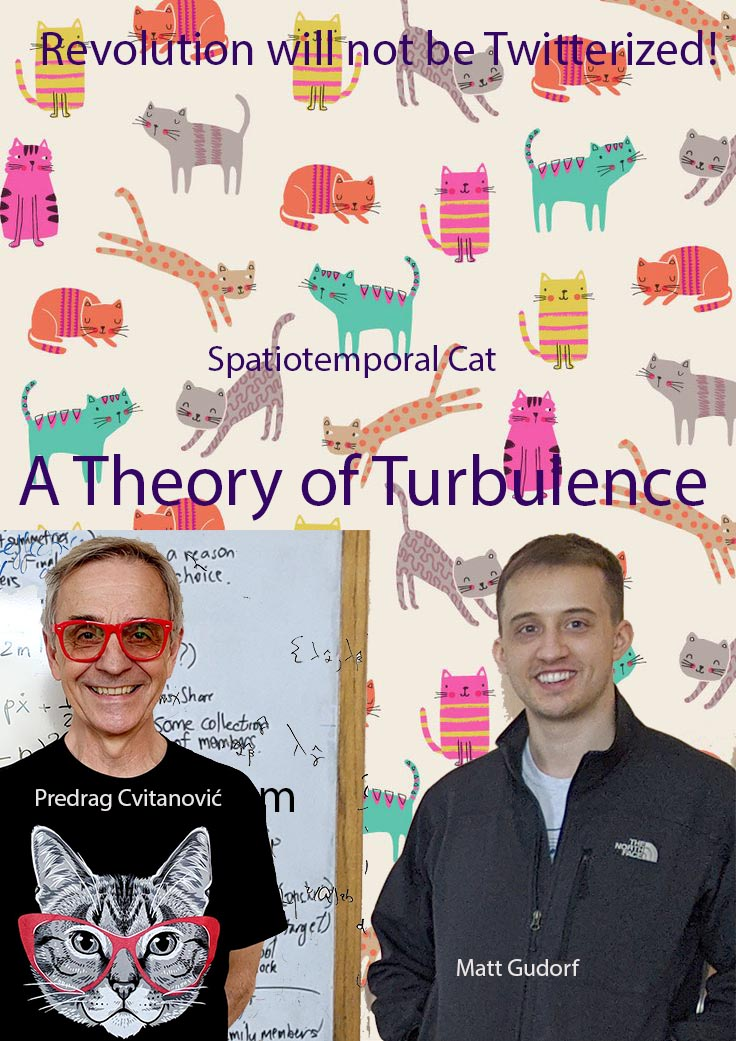
\includegraphics[width=0.55\textwidth]{HoweyCats}
\end{center}
\end{frame}

\begin{frame}
  \titlepage
\end{frame}


\section[what this work is about]
 {what this work is about}

\begin{frame}{overview}
\begin{enumerate}
              \item {\Large
what this talk is about
                  }\textcolor{gray}{\small
              \item
turbulence in large domains
              \item
space is time
              \item
bye bye, dynamics
                    }
            \end{enumerate}
\end{frame}

\begin{frame}{do clouds solve PDEs?}

%and do they care what PST hour is it?
%\\
%and at what longitude are they?
%\\
do clouds \textcolor{red}{integrate} Navier-Stokes equations?

\begin{center}
\centerline{\textcolor{red}{\Huge NO!}}
%\end{center}
%for weather prediction, we store sets of weather sequences
%\bigskip\bigskip

%\begin{center}
\begin{minipage}[t]{\textwidth}
	\begin{center}
%\vspace{2ex}
\centerline{
\raisebox{-4.0ex}[5.5ex][4.5ex]
		 {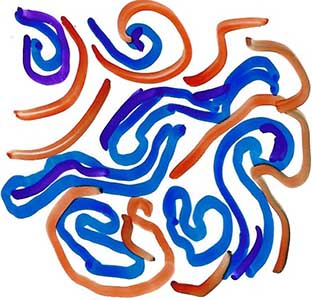
\includegraphics[height=12ex]{Hopf-a}}
~~~ $\Longrightarrow$ ~~ {other swirls} ~~ $\Longrightarrow$ ~~~
	\raisebox{-4.0ex}[5.5ex][4.5ex]
		 {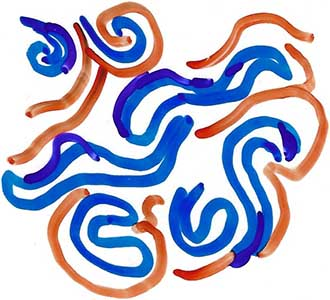
\includegraphics[height=12ex]{Hopf-b}}
          }
	\end{center}
\end{minipage}
\end{center}

do clouds satisfy Navier-Stokes equations?

\bigskip

{\Large yes!}

\centerline{
\textcolor{blue}{they satisfy them \textcolor{red}{\large locally}, everywhere and at all times}
}
\end{frame}

\begin{frame}{part 1}
\begin{enumerate}
              \item {\Large
turbulence in large domains
                  }\textcolor{gray}{\small
              \item
space is time
              \item
spacetime
              \item
bye bye, dynamics
                    }
            \end{enumerate}
\end{frame}


\begin{frame}{goal : enumerate the building blocks of turbulence}
\begin{block}{Navier-Stokes equations} % (1822)}
\[
\dfrac{\partial \bv}{\partial t} + (\bv \cdot \nabla) \bv
	\,=\,
\frac{1}{R} \nabla ^2 \bv
-\nabla p
+ \mathbf{f}
    \,,\qquad
\nabla \cdot \bv = 0,
\]
\end{block}

\hfill{\small
velocity field  $\bv \in \mathbb{R}^3$
;
pressure field $p$
;
driving force $\mathbf{f}$
        }

\medskip

\begin{block}{describe turbulence}
starting from the equations (no statistical assumptions)
\end{block}

\bigskip

% large Reynolds number $R$:
\hfill {\Large\textcolor{red}{}}

\end{frame}

\begin{frame}{challenge : experiments are amazing}
\begin{center}
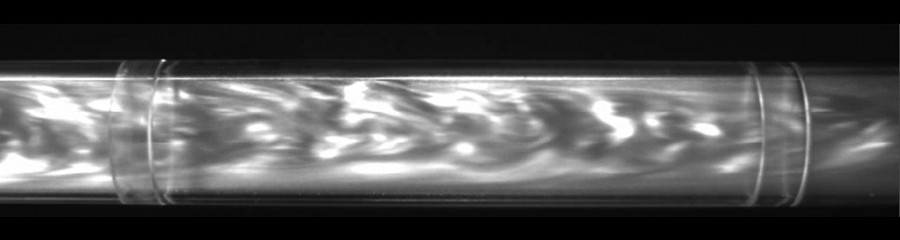
\includegraphics[width=0.7\textwidth]{mullin_puff2200} %pipe}
\end{center}
T. Mullin lab
\begin{center}
\bigskip
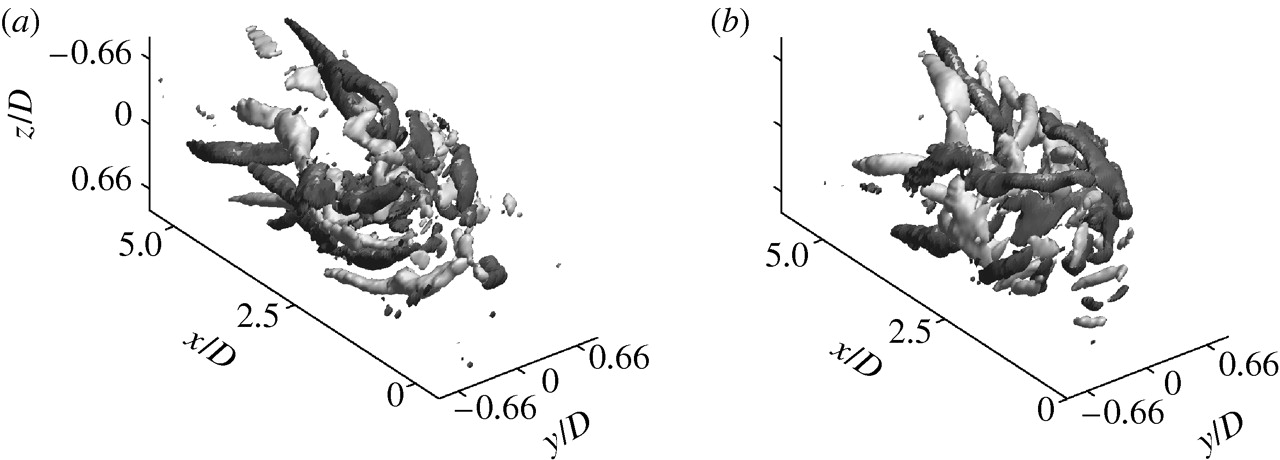
\includegraphics[width=0.7\textwidth]{deLHof09fig6} %pipe}
\end{center}
B. Hof lab
\end{frame}

%\begin{frame}{pipe theory and numerics}
%	\begin{columns}[t]
%	\column{.55\textwidth}
%amazing experiments! \\ amazing numerics! \\ beautiful visualizations !
%
%\bigskip\bigskip
%
%%relative periodic orbits,
%``Exact Coherent Structures'' :
%\\ numerical Navier-Stokes
%
%\medskip
%isosurfaces and cross sections \\ of the streamwise velocity
%
%\medskip
%
%\textcolor{red}{red} (\textcolor{blue}{blue}) streaks
%\\ are \textcolor{red}{faster} (\textcolor{blue}{slower}) \\ than the base flow
%
%\bigskip
%
%{{\tiny Ritter et al., Phys. Rev. Fluids (2018)}}
%
%	\column{.45\textwidth}
%\begin{center}
%  \includegraphics[width=1.0\textwidth,clip=true]
%                    {RZSEA18Fig3}
%\end{center}
%	\end{columns}
%\end{frame}

\section[dynamics in $\infty$ dimensions]
{dynamics in $\infty$ dimensions}

\begin{frame}{can simulate {\Huge large} computational domains}
\begin{center}
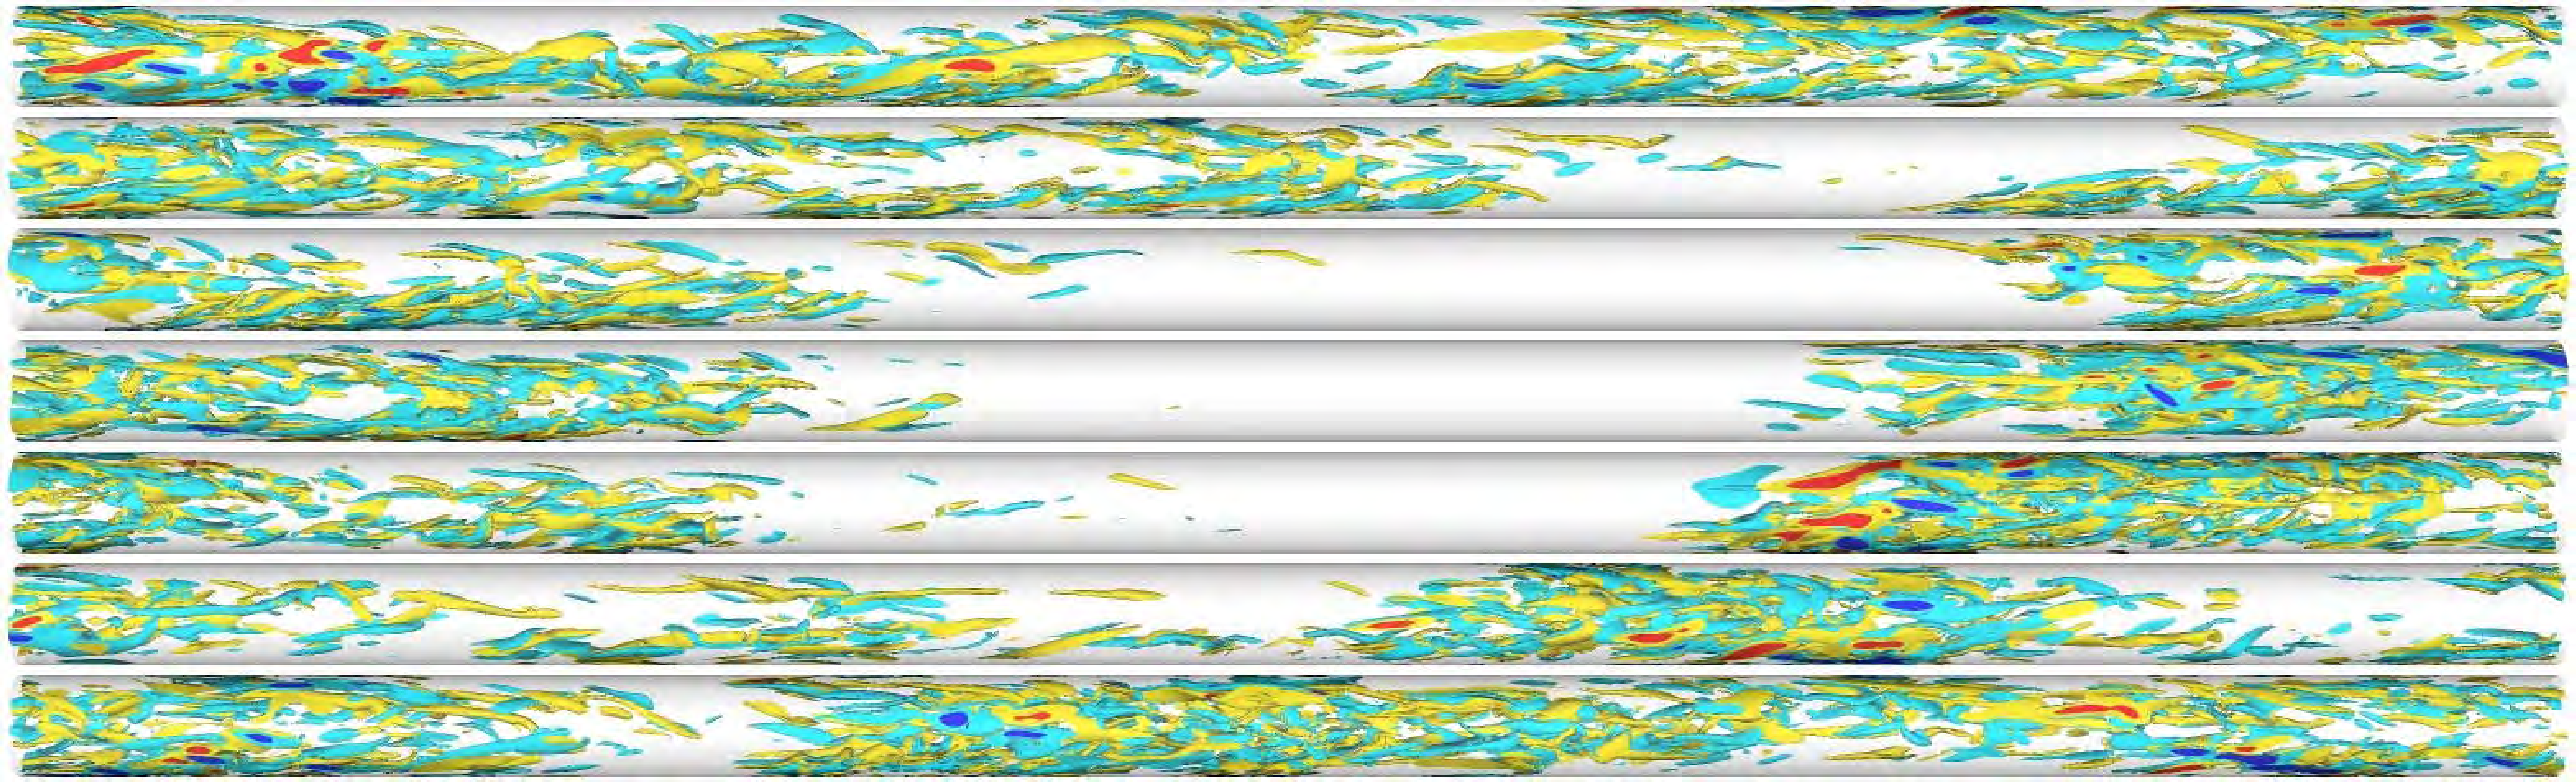
\includegraphics[width=1.0\textwidth]{AviHof13fig4}
\end{center}
pipe flow close to onset of turbulence
\footnote{M.~Avila and B.~Hof, {Phys. Rev. \bf E 87} (2013)}

\bigskip

but we have \textcolor{red}{\Huge hit a wall} :

\hfill exact coherent structures are too unstable to compute
\end{frame}

\begin{frame}{goal : we can do 3D turbulence, but for this talk}
\begin{block}{Navier-Stokes equations} % (1822)}
\[
\dfrac{\partial \bv}{\partial t} + (\bv \cdot \nabla) \bv
	\,=\,
\frac{1}{R} \nabla ^2 \bv + (\cdots)
% -\nabla p + \mathbf{f}
%    \,,\qquad
%\nabla \cdot \bv = 0,
\]
\end{block}

\hfill{\small velocity field  $\bv(\bx;t) \in \mathbb{R}^3$}

\medskip

\begin{block}{not helpful for developing intuition}
we cannot visualize 3D velocity field at every 3D spatial point
\end{block}

\bigskip

% large Reynolds number $R$:
\hfill {\Large\textcolor{red}{look instead at 1D `flame fronts'}}
\end{frame}

\begin{frame}{(3+1) spacetime dimensional ``Navier-Stokes''}
\begin{block}{Navier-Stokes equations \hfill (1822)}
\[
\dfrac{\partial \bv}{\partial t} + (\bv \cdot \nabla) \bv
	\,=\,
\frac{1}{R} \nabla ^2 \bv + (\cdots)
\]
\end{block}
    \centerline{\textcolor{red}{$\blacktriangledown$}}
    \centerline{\textcolor{red}{$\blacktriangledown$}}
    \centerline{\textcolor{red}{$\blacktriangledown$}}
\begin{block}{\KS\ (1+1)\dmn\ PDE \hfill (1975)}
\[
  u_t + u \triangledown u \,=\,
    {\color{red}-}\triangledown^2 u {\color{red}-\triangledown^4 u}
    \,,\qquad   x \in \mathbb{R}
    \,,
\]
\end{block}
\bigskip

describes spatially extended systems such as
\begin{itemize}
 \item flame fronts in combustion
 \item reaction-diffusion systems
 \item \ldots
\end{itemize}
\end{frame}

\begin{frame}{an example : \KS\ on a large domain}
\begin{center}
  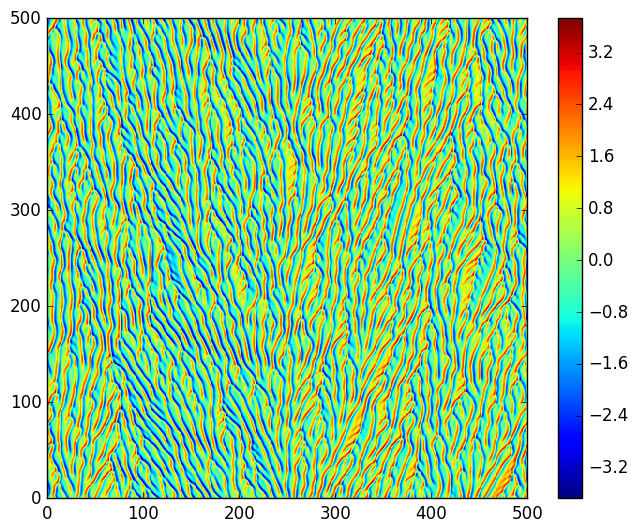
\includegraphics[width=.6\textwidth]{MNG_uu500b500}
%  \includegraphics[width=0.6\textwidth] %,height=0.5\textheight,clip=true]
%  {ks_largeL_cbar_200} %{ksevol-fig} %{ks_largeL_cbar}
\end{center}

{\footnotesize
[horizontal] space $\ssp \in [0,L]$
\qquad
{[up]} time evolution
}

\begin{itemize}
\item turbulent behavior
\item simpler physical, mathematical and computational setting than Navier-Stokes
\end{itemize}
\end{frame}

\begin{frame}{compact space, infinite time cylinder}
\begin{center}
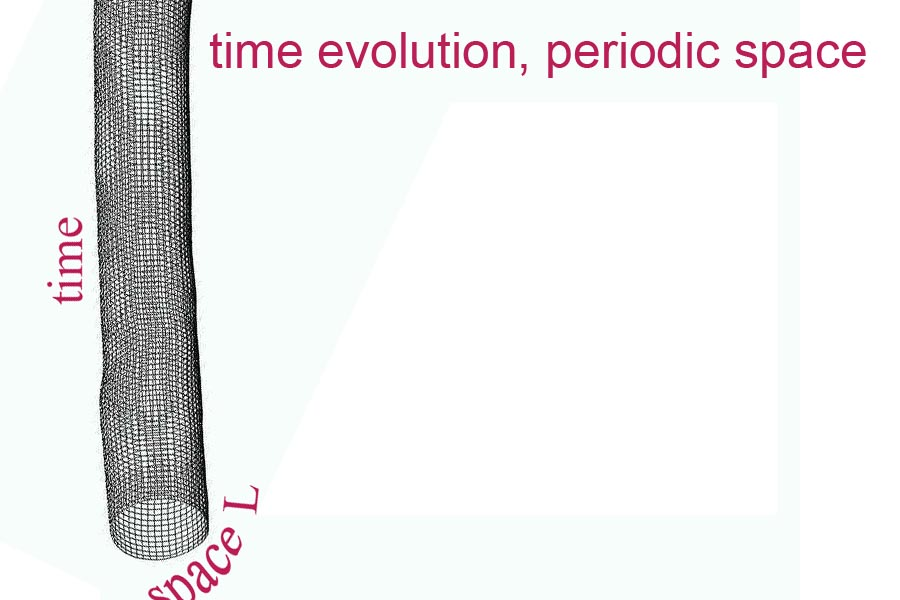
\includegraphics[width=0.9\textwidth]{cylinderTime}
\end{center}
% \hfill \color{red}{(impossible without xxx)}
so far : Navier-Stokes on compact spatial domains, all times
\end{frame}

\begin{frame}{compact space, infinite time} % \KS}
\begin{block}{\KS\ equation}
\[
  u_t \,=\,
    -({\color{red}+}\triangledown^2 +{\color{red}\triangledown^4}) u
    - u \triangledown u
    \,,\qquad   x \in [-L/2,L/2]
    \,,
\]
\end{block}

\bigskip

\begin{block}{in terms of discrete spatial Fourier modes}
$N$ ordinary differential equations (ODEs) in time
\[
\dot{\Fu}_k(\zeit) = ( q_k^2 - q_k^4 )\, \Fu_k(\zeit)
- i \frac{q_k}{2} \!\sum_{k'=0}^{N-1} \!\!\Fu_{k'}(\zeit) \Fu_{k-k'}(\zeit)
\,.
%\label{e-Fks}
\]
\end{block}
\end{frame}


\subsection{types of solutions}
\begin{frame}{evolution of \KS\ on small $L=22$ cell}
\begin{center}
  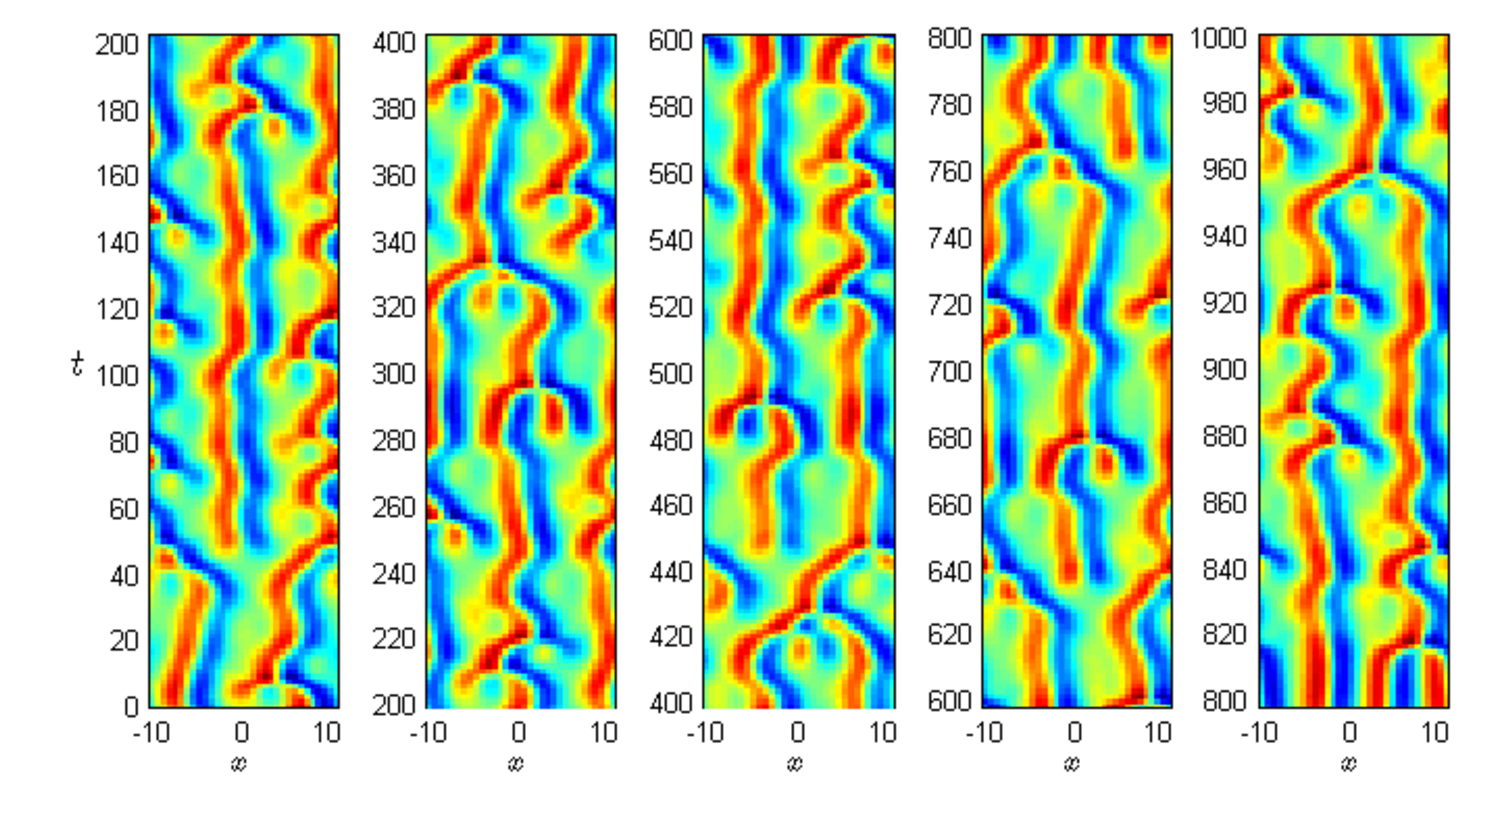
\includegraphics[width=0.9\textwidth,clip=true]{ks_L22_long_orbit}
\end{center}
horizontal: $x \in [-11,11]$
\\
vertical: time
\\
color: magnitude of 1D velocity $u(x,t)$
\end{frame}

\begin{frame}{part 2}
\begin{enumerate}
              \item
    \textcolor{gray}{\small
turbulence in large domains
        }
              \item
    {\Large
space is time
    }\textcolor{gray}{\small
              \item
spacetime
              \item
bye bye, dynamics
                    }
            \end{enumerate}
\end{frame}

\begin{frame}{yes, but}
\begin{center}
{\huge is space time?}
\end{center}
\end{frame}

\begin{frame}{compact time, infinite space}
rewrite \KS
\bea
    u_\zeit &=&  - u u_\conf
    -u_{\conf \conf}-u_{\conf \conf \conf \conf}
\nonumber     % \label{e-ks}
\eea
 as  4-fields vector
\bea
\transp{{\bf u}}&=&(u,u^{'},u^{''},u^{'''})
    \continue
&& \mbox{where }
    u^{'}   \equiv u_{\conf} \,,\;
    u^{''}  \equiv u_{\conf \conf} \,,\;
    u^{'''} \equiv u_{\conf \conf \conf}
\nnu
\eea
equation
\(
\frac{d~}{d\conf}{\bf u}(x)={\bf v}(x)
\)
now {\color{blue}1st order} in {\color{blue}spatial} derivative
\begin{block}{\KS\ = four coupled 1st order PDEs}
\bea
    \frac{d\,u}{d\conf}       &=& u^{'}
\,,\qquad
    \frac{d\,u^{'}}{d\conf}   \,=\,   u^{''}
\continue
    \frac{d\,u^{''}}{d\conf~}   &=&   u^{'''}
\,,\qquad
    \frac{d\,u^{'''}}{d\conf~~}  \,=\,  - u_{\zeit} - u^{''} - u\,u^{'}
\nonumber
\eea
\end{block}
\end{frame}

\begin{frame}{compact time, infinite space}
  1st order in {\color{blue}spatial} derivative
\begin{block}{evolve four 1st order PDEs for ${\bf u}(x)$ in $\conf$,}
\begin{itemize}
  \item
\[
\frac{d~}{d\conf}{\bf u}(x)={\bf v}(x)
\]
  \item
periodic boundary condition in time
\[
  u(\conf, \zeit) = u(\conf, \zeit + \period{})
\]
  \item
initial data
\[
  \transp{{\bf u}}_0=(u(\conf_0, \zeit),u^{'}( \conf_0, \zeit),
                      u^{''}( \conf_0, \zeit),u^{''}( \conf_0, \zeit))
\]
specified for all $\zeit \in [0, \period{})$, at a fixed space point $\conf_0$
\end{itemize}
\end{block}
\end{frame}

\begin{frame}{a solution integrated in either time or space}
\begin{center}
  \begin{minipage}[height=.40\textheight]{.35\textwidth}
    \centering \small{\texttt{(left)}}
    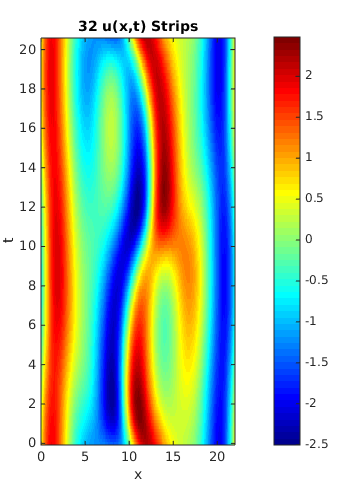
\includegraphics[width=\textwidth,height=.60\textheight]{MNGcomp32xint22}
  \end{minipage}
~~~~~~~~~
  \begin{minipage}[height=.40\textheight]{.35\textwidth}
    \centering \small{\texttt{(right)}}
    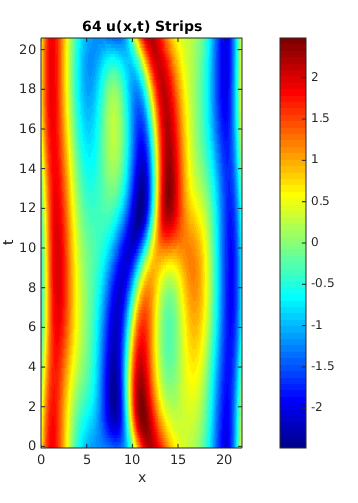
\includegraphics[width=\textwidth,height=.60\textheight]{MNGcomp64xint22}
  \end{minipage}
\end{center}
    (left) old : time evolution. (right) new : space evolution
    \\
    $x=[0,L]$ %22]$,
       initial condition : time periodic line $t = [0,T]$
  %2\,T_{\PPO{10.2}})$
  %\label{fig:MNGcompxint2}

\vfill\hfill        Gudorf 2016
\end{frame}

\begin{frame}{can do : compact time, infinite space cylinder}
\begin{center}
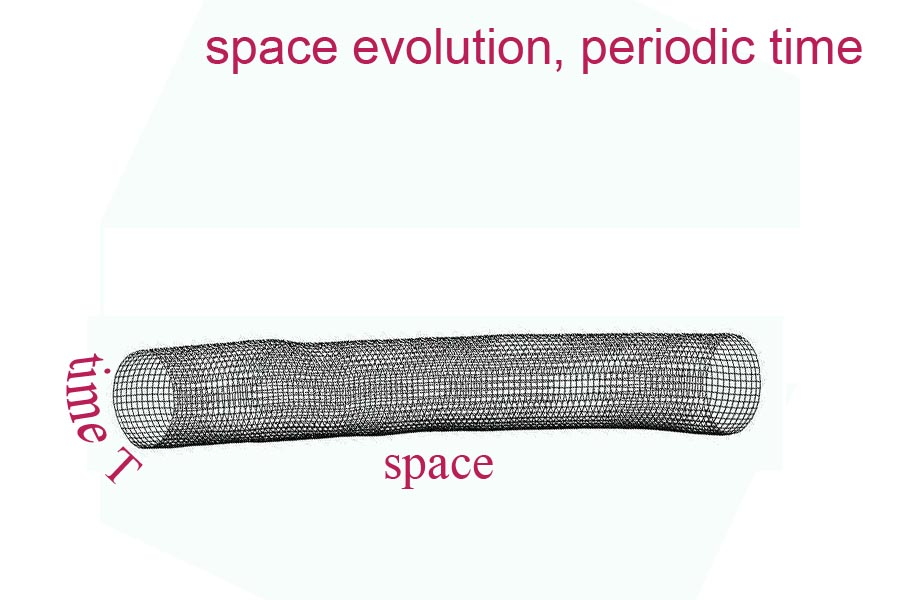
\includegraphics[width=0.9\textwidth]{cylinderSpace}
\end{center}
% \hfill \color{red}{(impossible without xxx)}
\end{frame}

\begin{frame}{but integrations are uncontrollably unstable}
\begin{center}
{\huge neither} time {\huge nor} space integration {\huge works} \\
for large domains
\end{center}

\vfill
\color{red}{rethink the formulation!}
\end{frame}

\begin{frame}{part 3}
\begin{enumerate}
              \item
    \textcolor{gray}{\small
turbulence in large domains
              \item
space is time
    }
              \item {\Large
spacetime
    }\textcolor{gray}{\small
              \item
bye bye, dynamics
                    }
            \end{enumerate}
\end{frame}

\begin{frame}
    \frametitle{\KS\ on a large spacetime domain}
\begin{block}{the same small tile recurs often in a turbulent pattern}
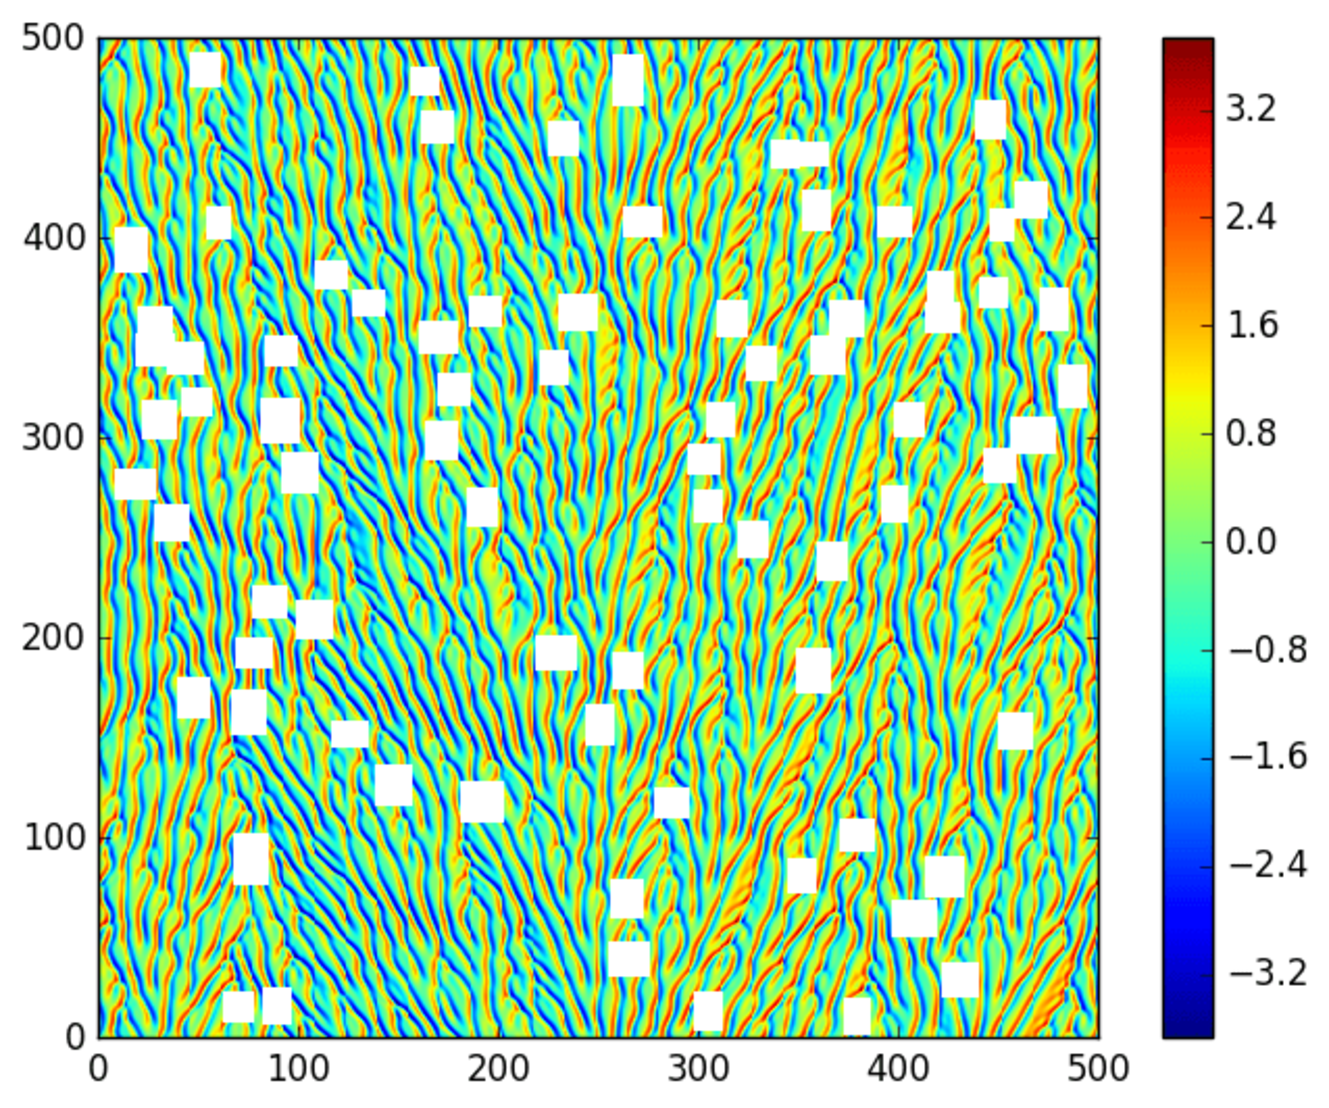
\includegraphics[width=.48\textwidth]{MNG_uu500b500co}
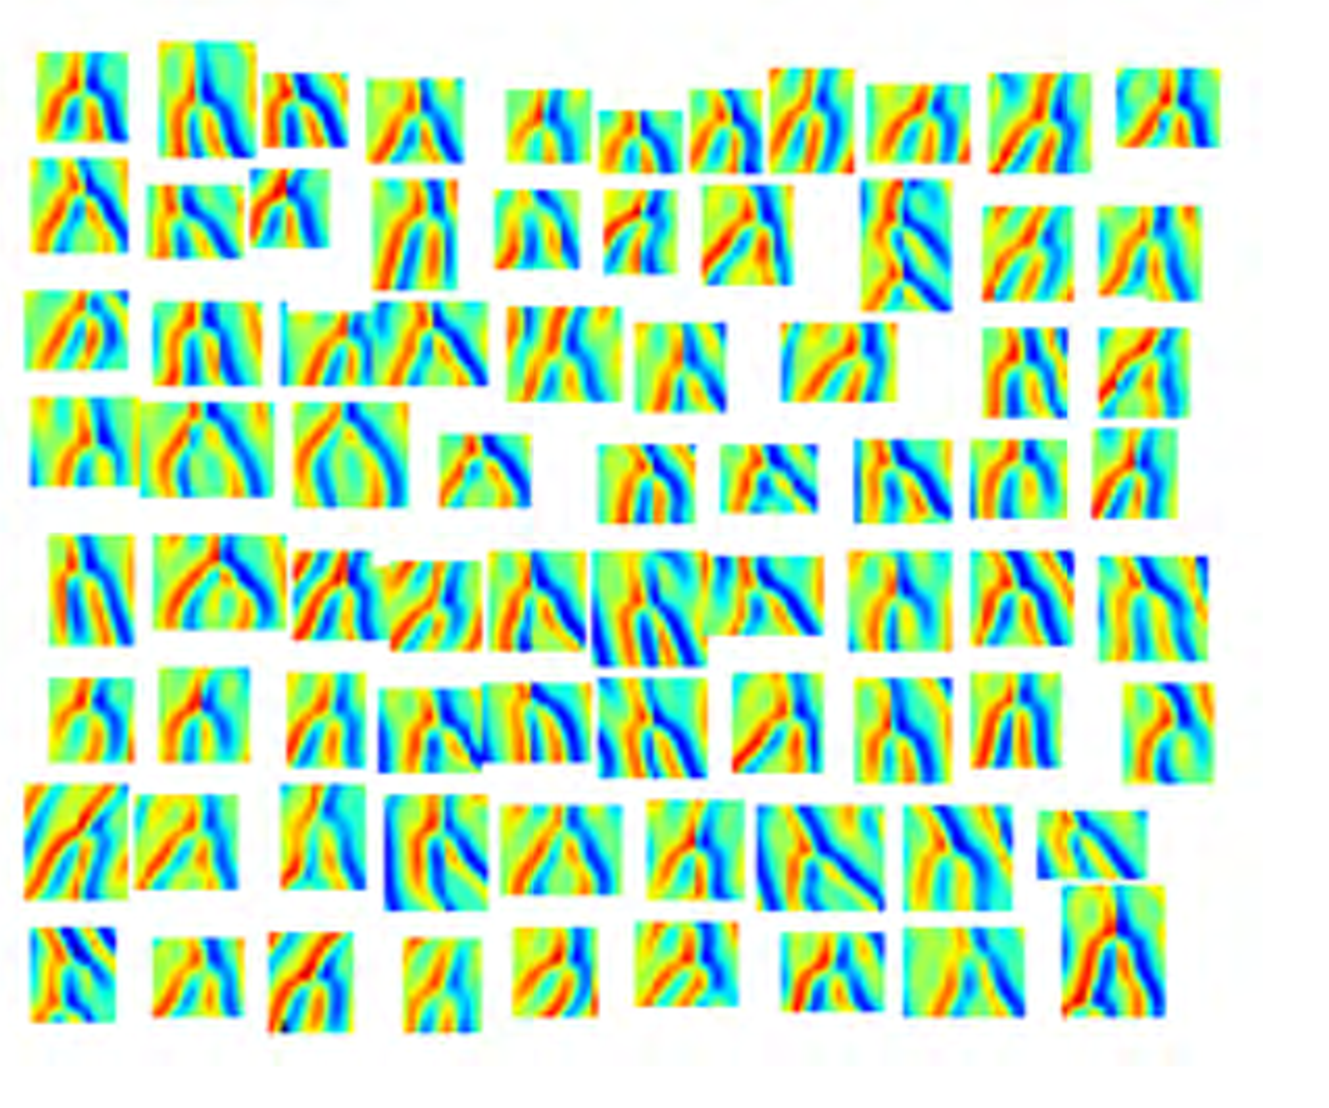
\includegraphics[width=.48\textwidth]{cutouts}
\end{block}
goal : define, enumerate nearly recurrent tiles
\vfill\hfill        Gudorf 2018
\end{frame}

\begin{frame}{use spatiotemporally compact solutions as spacetime `tiles'}
\begin{center}
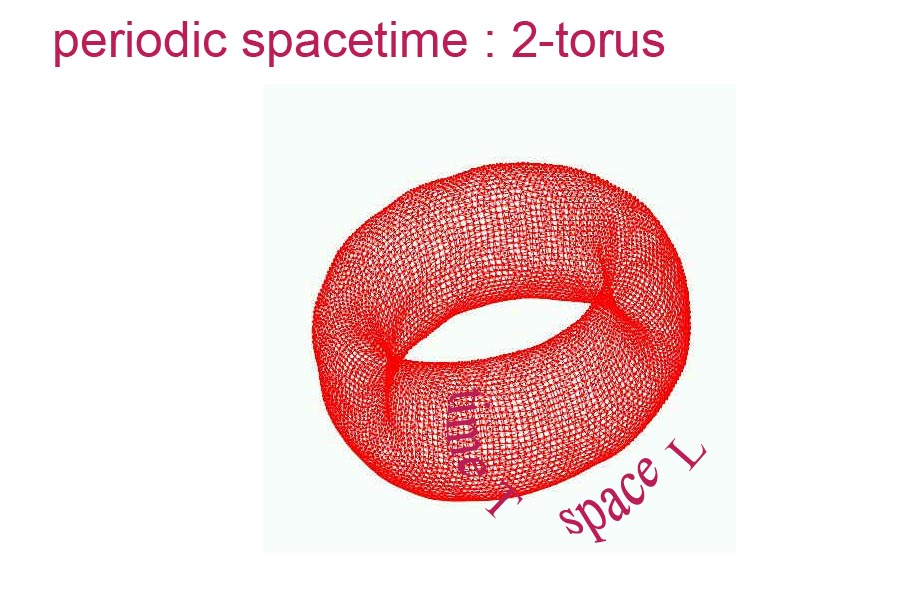
\includegraphics[width=0.9\textwidth]{torusSpTime}
\end{center}
\textcolor{red}{shadows} a small patch of spacetime
% \hfill \color{red}{(impossible without xxx)}
\end{frame}

\begin{frame}{\po s generalize to $d$-tori}

\begin{block}{1 time, 0 space dimensions}
a {\statesp} point is {\em periodic} if its orbit returns to it
after a finite time \period{} ;
\\
such orbit tiles the time axis
by infinitely many repeats
\end{block}

\bigskip

\begin{block}{1 time, $d$-1 space dimensions}
 a {\statesp} point is {\em spatiotemporally periodic} if
it belongs to \\ an invariant $d$-torus ${\R}$ ;
\\
such torus tiles the spacetime
by infinitely many repeats
%,\\
%\ie, a \brick\ $\Mm_{\R}$ that
%tiles the lattice state  $\Mm$, \\
%with period $\ell_j$ in $j$th lattice direction
\end{block}
\end{frame}

\begin{frame}{every compact solution is a fixed point on a discrete lattice}
discretize $u_{nm} = u(\conf_n,\zeit_m)$ over
$N M$ points of spatiotemporal periodic lattice $\conf_n = n L/N$,
 $\zeit_m = m \period{}/M$, Fourier transform :
\[
\Fu_{k\ell} \,=\,
  \frac{1}{NM} \sum^{N-1}_{n=0} \sum^{M-1}_{m=0}
  u_{nm} \, e^{-i(q_k\conf_n + \omega_\ell \zeit_m)}
    \,,\quad
q_k = \frac{2 \pi k}{L}
    \,,\;
\omega_\ell = \frac{2 \pi \ell}{\period{}}
% \label{spattempFT}
\]
\KS\ is no more a PDE, \\
but an {\color{blue}{algebraic}} $[N\!\times\!M]$\dmn\ problem\\
of determining {\color{blue}{global}} solution ${\bf u}$ to
\begin{block}{fixed point condition}
\[
\left(- i \omega_\ell - ( q_k^2 - q_k^4 ) \right)\Fu_{k\ell}
+ i \frac{q_k}{2} \!\sum_{k'=0}^{N-1} \sum^{M-1}_{m'=0}\!\!
\Fu_{k'm'} \Fu_{k-k',m-m'}
    = 0
\]
\end{block}
\end{frame}

\begin{frame}{professor Zweistein forgets to take his meds}
\medskip
statement : {\huge HA!} \\
You are imposing by hand the space \& time periods
\speriod{}, \period{} {\huge !}

\begin{center}
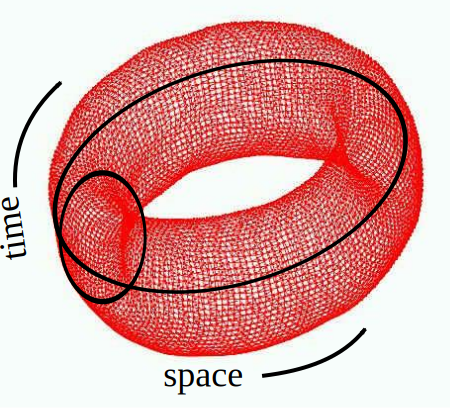
\includegraphics[width=0.35\textwidth]{spaceTime1}
\end{center}

answer : {\huge\color{red}{NO!}} \\
nature chooses \speriod{} \& \period{},
they are free parameters.
\end{frame}

\begin{frame}{every calculation is a spatiotemporal lattice calculation}
field is discretized as
$\Fu_{k\ell}$ values  \\ over
$N M$ points of a periodic lattice

%\medskip

\begin{center}
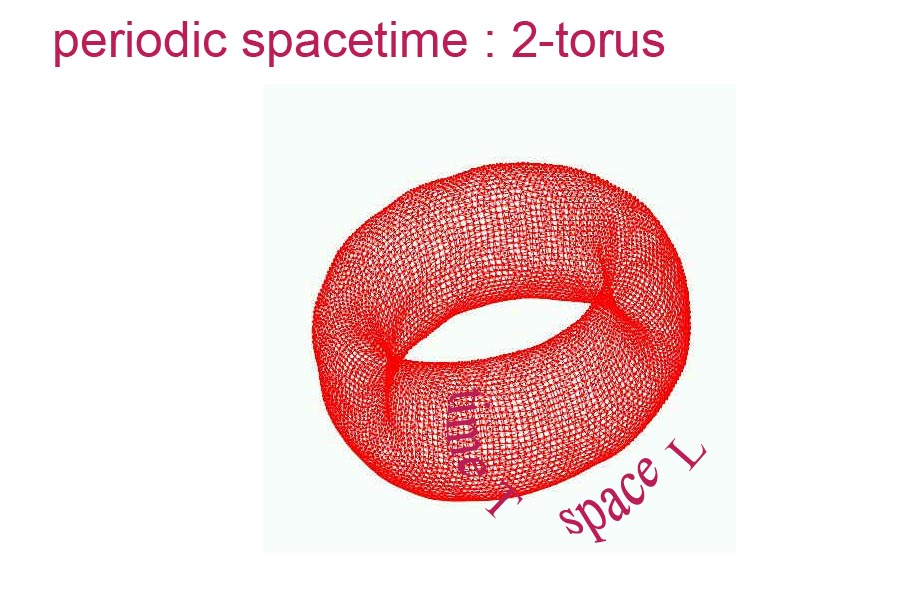
\includegraphics[width=0.9\textwidth]{torusSpTime}
\end{center}
% \hfill \color{red}{(impossible without xxx)}
\end{frame}


\begin{frame}{there is no more time evolution}
solution to \KS\ is now given as
\begin{block}{condition that}
at each lattice point $k\ell$ \\
the tangent field at $\Fu_{k\ell}$
\end{block}
satisfies the equations of motion
\[
\left[- i \omega_\ell - ( q_k^2 - q_k^4 ) \right]\Fu_{k\ell}
+ i \frac{q_k}{2} \!\sum_{k'=0}^{N-1} \sum^{M-1}_{m'=0}\!\!
\Fu_{k'm'} \Fu_{k-k',m-m'}
    =
0
%\,.
%\label{e-FksSpattemp}
\]

\bigskip

this is a \textcolor{red}{local} tangent field constraint on a
\textcolor{red}{global} solution
\end{frame}

\begin{frame}{think globally, act locally}
    \begin{center}
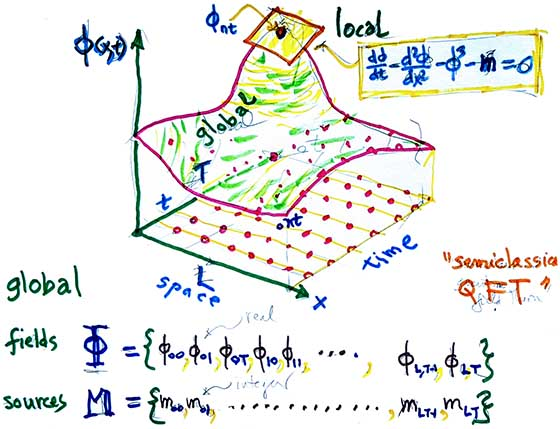
\includegraphics[width=0.85\textwidth]{globalLocal}
    \end{center}
for each symbol array \Mm, a periodic lattice state $\Xx_\Mm$
\end{frame}

\begin{frame}{unexpected gift from nature}
robust : no exponential instabilities
\\
\hfill as there are no finite time / space integrations
\bigskip

no need for $\sim
10^{-11}$ accuracies,
\bigskip

{\huge \textcolor{red}{so}}
\bigskip

accuracy to a few \% suffices, \\
\hfill you only need to get the shape of a solution right
\end{frame}

\begin{frame}{part 4}
\begin{enumerate}
              \item
    \textcolor{gray}{\small
turbulence in large domains
              \item
space is time
              \item
spacetime    }
              \item {\Large
spacetime computations
    }\textcolor{gray}{\small
              \item
bye bye, dynamics
                    }
            \end{enumerate}
\end{frame}


\begin{frame}{how to find solutions ? an ODE example}
\begin{center}
the law of motion : $\qquad \dot{\ssp} = \pVeloc(\ssp)$
\begin{minipage}[c]{0.55\textwidth}
\textcolor{red}{guess loop tangent}
$\lVeloc(\lSpace)
	\neq
\pVeloc(\lSpace)$

	\vskip 0.5cm

\textcolor{green}{periodic orbit}
$\lVeloc(\lSpace)$,~$\pVeloc(\lSpace)$
aligned
\end{minipage}%
~~~~~~~\begin{minipage}[c]{0.40\textwidth}
	\begin{center}
	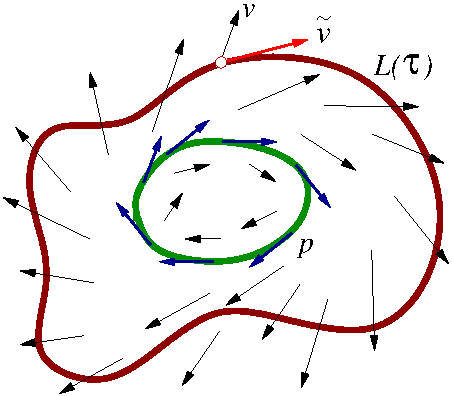
\includegraphics[width=0.7\textwidth]{velocField}
	\end{center}
\end{minipage}
\end{center}
\begin{block}{cost function}%
\[
\costF[\lSpace] =
            \oint_\Loop ds\,(\lVeloc-\pVeloc)^2
    \,;\quad
    \lVeloc = \lVeloc(\lSpace(s,\tau))\,,\,\,
    \pVeloc = \pVeloc(\lSpace(s,\tau))
\,,
% \label{loopCostFct}
\]
\end{block}
\bigskip

penalize\footfullcite{lanVar1} %{ Lan and Cvitanovi\'c, Phys. Rev. (2004)}
 misorientation of the loop tangent
$\lVeloc(\lSpace)$
relative to the true dynamical flow tangent field $\pVeloc(\lSpace)$
\end{frame}

\begin{frame}{how do clouds solve PDEs?}
clouds do not \textcolor{red}{\Huge NOT} {integrate} Navier-Stokes equations

\bigskip\bigskip

\begin{center}
\begin{minipage}[t]{\textwidth}
	\begin{center}
\centerline{
\raisebox{-4.0ex}[5.5ex][4.5ex]
		 {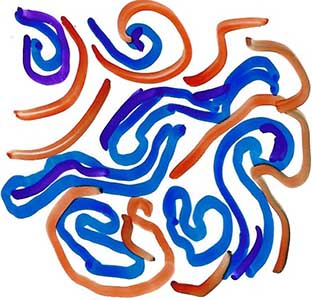
\includegraphics[height=12ex]{Hopf-a}}
~~~ $\Longrightarrow$ ~~ {other swirls} ~~ $\Longrightarrow$ ~~~
	\raisebox{-4.0ex}[5.5ex][4.5ex]
		 {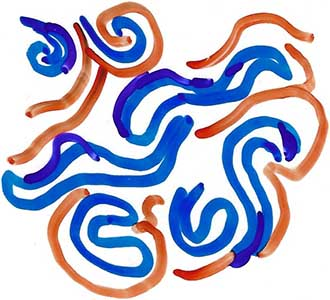
\includegraphics[height=12ex]{Hopf-b}}
          }
	\end{center}
\end{minipage}
\end{center}

do clouds satisfy Navier-Stokes equations?

\bigskip

{\Large yes!}

\centerline{
\textcolor{blue}{they satisfy them \textcolor{red}{\large locally}, everywhere and at all times}
}
\end{frame}

\begin{frame}{the equations imposed as local constraints}
\begin{block}{\KSe}
\[
F(u) = u_t + u_{\conf \conf} + u_{\conf \conf \conf \conf} + u u_{\conf} = 0
\]
\end{block}
\bigskip\bigskip
for example, minimize
\begin{block}{cost function}
\[
G \equiv \frac{1}{2} |F(u)|^2_{L \times T}
%\ee{costfunctional}
\]
\end{block}
\vfill\hfill\textcolor{red}{\Huge need your help !}
\end{frame}

\begin{frame}{does this work ?}
add strong noise to a \emph{known} solution, \\ twice the typical amplitude
\begin{block}{only the first test}
{\scriptsize (not how we actually generate guesses)} \\
\begin{minipage}[height=.32\textheight]{.35\textwidth}
\centering %\small{\texttt{(a)}}
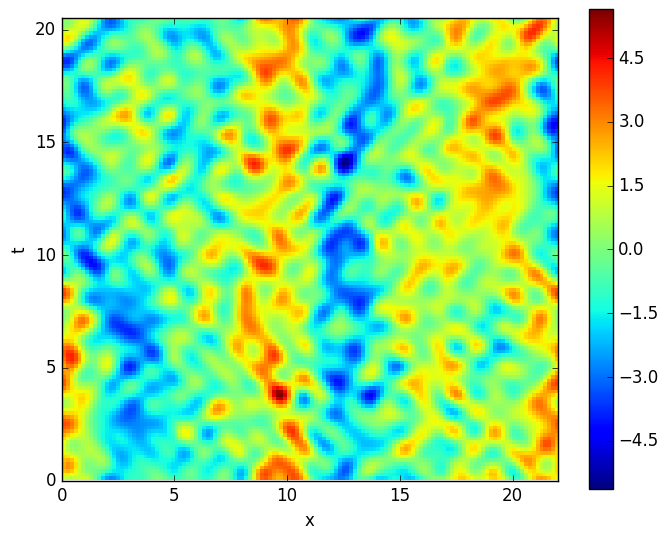
\includegraphics[width=\textwidth,height=.32\textheight]{MNG_ppo1_noise_init}
\end{minipage}
    \qquad
\begin{minipage}[height=.32\textheight]{.35\textwidth}
\centering %\small{\texttt{(right)}}
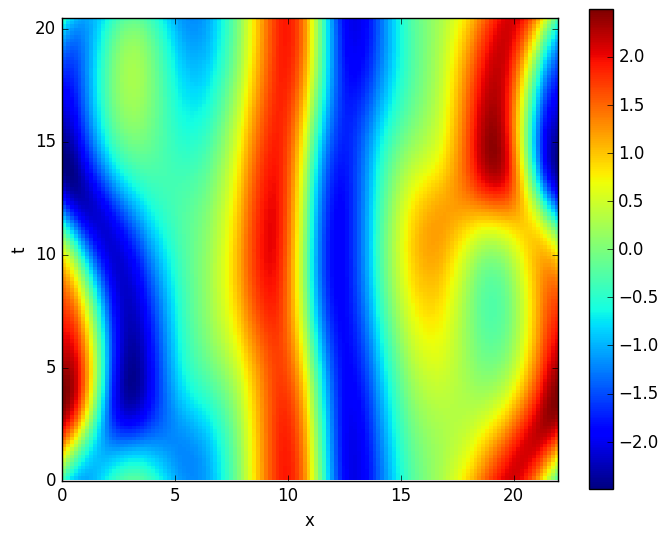
\includegraphics[width=\textwidth,height=.32\textheight]{MNG_ppo1_noise_conv}
\end{minipage}
%\caption{ \label{fig:MNG_adjnewt_robustness}
\end{block}

{\scriptsize (left) initial guess: a known %\PPO{10.2}
\twot} \\
$(\speriod{0},\period{0})=(22.0,20.5057459345)$
+
strong random noise
\medskip

{\scriptsize (right) the resulting adjoint descent converged \twot} \\
$(\speriod{f},\period{f})=(21.95034935834641,20.47026321555662)$
%\end{figure}
\end{frame}

\begin{frame}{KS \twot\ found variationally}
%%%%%%%%%%%%%%%%%%%%%%%%%%%%%%%%%%%%%%%%%%%%%%%%%%%%%%%%%%%%%%%%
%\label{fig:MNG_spacetime_smoothed} from siminos/spatiotemp/blogMNG.tex
\begin{minipage}[height=.72\textheight]{.40\textwidth}
\centering \small{\texttt{(left)}}
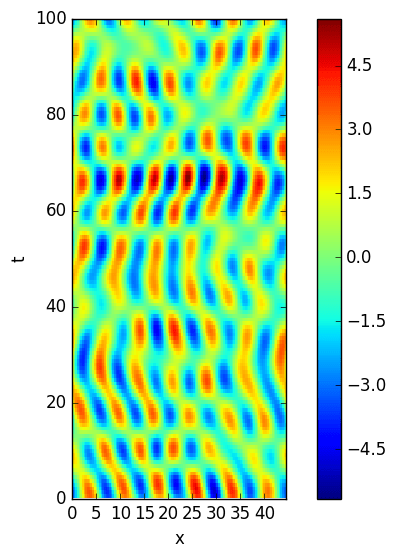
\includegraphics[width=\textwidth,height=.63\textheight]{MNG_T100L44_init}
\end{minipage}
\begin{minipage}[height=.72\textheight]{.40\textwidth}
\centering \small{\texttt{(right)}}
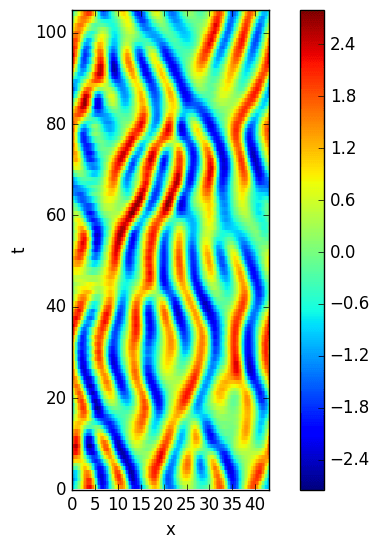
\includegraphics[width=\textwidth,height=.63\textheight]{MNG_T100L44_final}
\end{minipage}

\vfill
(left) initial : $\bar{L}=2\pi\sqrt{2}$ spatially modulated ``noisy'' guess

(right) adjoint descent : converged \twot\
% \\
% spatial and time periods
% $L=24.07$, $T=31.86$
%%%%%%%%%%%%%%%%%%%%%%%%%%%%%%%%%%%%%%%%%%%%%%%%%%%%%%%%%%%%%%%%

\vfill\hfill        Gudorf 2018
\end{frame}

\begin{frame}{our guesses are extracted from large spacetime domains}
\begin{minipage}[height=.45\textwidth]{.45\textwidth}
\centering %\small{\texttt{(a)}}
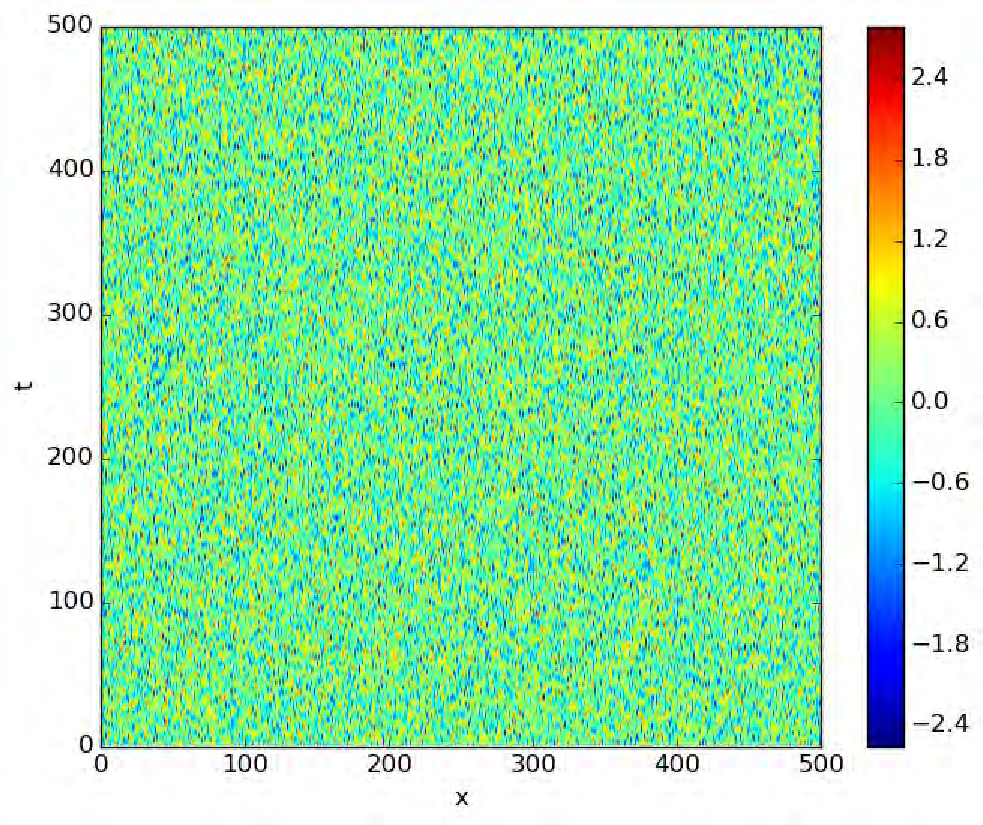
\includegraphics[width=\textwidth,height=.45\textheight]{MNGadjdescent500b500init}
\end{minipage}
\begin{minipage}[height=.45\textwidth]{.45\textwidth}
\centering %\small{\texttt{(b)}}
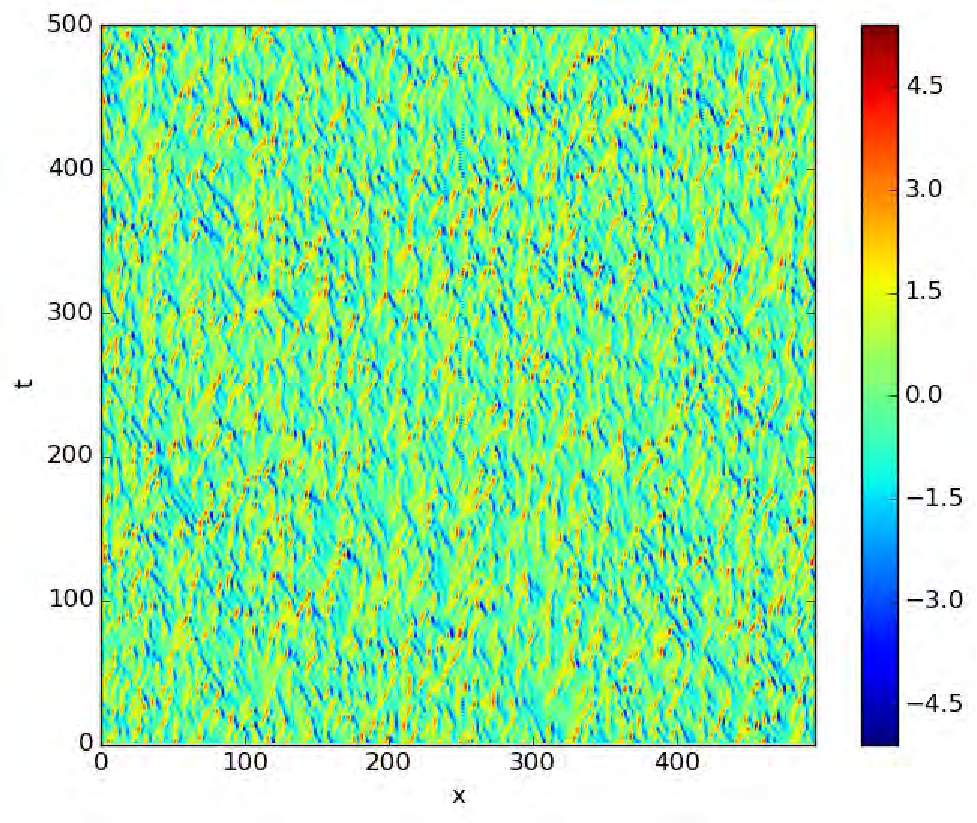
\includegraphics[width=\textwidth,height=.45\textheight]{MNGadjdescent500b500fin}
\end{minipage}
%\caption{ \label{fig:MNGlarge_adjointdescent}

(left) random initial state on
%\hfill
$(L_0,T_0)=(500.0,500.0)$

(right) adjoint descent $\to$ typical \KS\ state

\vfill\hfill
finite windows are starting guesses for \twots
\end{frame}

\begin{frame}{embarrassment of riches}
\begin{center}
{\huge what to do?}
\end{center}

\vfill

{\Large Matt Gudorf}

\medskip

\hfill has 1,000's of such \twots
\end{frame}


\begin{frame}{part 5}
\begin{enumerate}
              \item
    \textcolor{gray}{\small
turbulence in large domains
              \item
space is time
              \item
spacetime
    }
              \item {\Large
fundamental tiles
    }\textcolor{gray}{\small
              \item
bye bye, dynamics
                    }
            \end{enumerate}
\end{frame}


\begin{frame}{building blocks of turbulence}

how do we \textcolor{red}{recognize} a cloud?

\bigskip
\begin{center}
\centerline{\textcolor{red}{\Huge WATCH}}
%\end{center}
%for weather prediction, we store sets of weather sequences
%\bigskip\bigskip

%\begin{center}
\begin{minipage}[t]{\textwidth}
	\begin{center}
%\vspace{2ex}
\centerline{
\raisebox{-4.0ex}[5.5ex][4.5ex]
		 {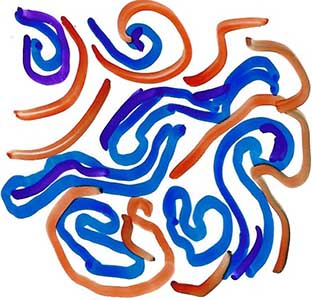
\includegraphics[height=12ex]{Hopf-a}}
~~~ $\Longrightarrow$ ~~ {other swirls} ~~ $\Longrightarrow$ ~~~
	\raisebox{-4.0ex}[5.5ex][4.5ex]
		 {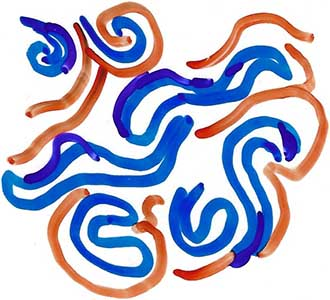
\includegraphics[height=12ex]{Hopf-b}}
          }
	\end{center}
\end{minipage}
\end{center}

\bigskip

{\Large by recurrent shapes!}

\vfill

\centerline{
\textcolor{blue}{so, construct an \textcolor{red}{\Large alphabet} of possible shapes}
}
\end{frame}

\begin{frame}{extracting a fundamental tile}
\begin{minipage}[height=.60\textheight]{.24\textheight}
\centering % \small{\texttt{(a)n}}
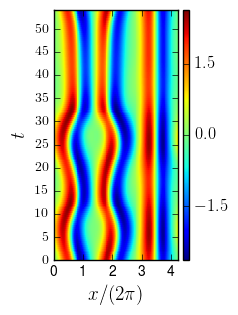
\includegraphics[width=.3\textheight,height=.55\textheight]{MNG_gapfull}
\end{minipage} \quad
\begin{minipage}[height=.60\textheight]{.24\textheight}
\centering % \small{\texttt{(b)}}
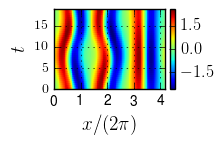
\includegraphics[width=.3\textheight,height=.25\textheight]{MNG_gapsub1}
\end{minipage} \quad
\begin{minipage}[height=.60\textheight]{.18\textheight}
\centering             % \small{\texttt{(c)}}
\includegraphics[width=0.26\textheight,height=.27\textheight]{MNG_gap}
\end{minipage} \quad
\begin{minipage}[height=.60\textheight]{.12\textheight}
\centering % \small{\texttt{(d)}}
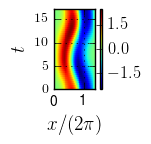
\includegraphics[width=0.17\textheight,height=.21\textheight]{MNG_gap_final}
\end{minipage}
%\label{fig:MNG_catseyefigs}

1) \twot\ %full\_L26.7\_T54.
    \\
2) \twot\ computed from initial guess cut out from 1)
    \\
3) ``gap" \twot, % po\_L17.3\_T15.3  %\reffig{fig:MNG_ppo_subdomains},
     initally cut out from 2)
     \\
4) the ``gap"  prime  \twot\ fundamental domain
\end{frame}

\begin{frame}%[allowframebreaks]
  \frametitle{a trial set of prime (rubber) tiles}
  \begin{block} {an alphabet of \KS\ fundamental tiles}
\begin{minipage}[height=.60\textheight]{.25\textheight}
\centering             % \small{\texttt{(c)}}
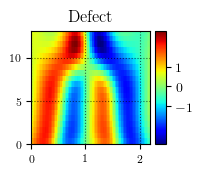
\includegraphics[width=0.26\textheight,height=.27\textheight]{ksstFigs/MNG_defect}
\end{minipage} \qquad
  % 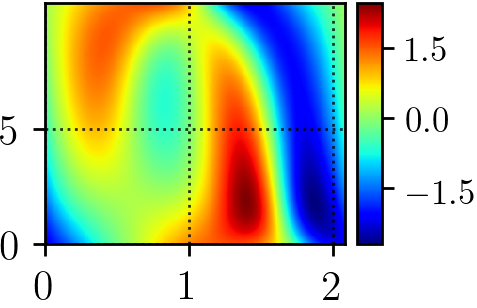
\includegraphics[width=.2\textwidth]{MNG_hook}
  % 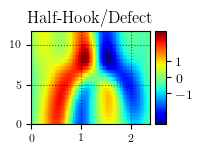
\includegraphics[width=.2\textwidth]{MNG_half}
\begin{minipage}[height=.60\textheight]{.25\textheight}
\centering     %{\footnotesize\texttt{\quad\quad Gap}}
\includegraphics[width=0.26\textheight,height=.27\textheight]{ksstFigs/MNG_gap}
\end{minipage} \qquad
\begin{minipage}[height=.60\textheight]{.25\textheight}
\centering             % \small{\texttt{(c)}}
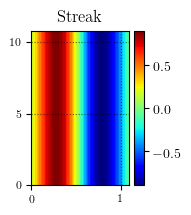
\includegraphics[width=0.25\textheight,height=0.25\textheight]{ksstFigs/MNG_streak}
\end{minipage}
  \end{block}
\vfill
utilize also discrete symmetries : \\
spatial reflection, spatiotemporal shift-reflect,
$\cdots$
\end{frame}

\begin{frame}{spacetime tiled by a small tile}
  \includegraphics[width=0.7\textwidth] %,height=0.5\textheight,clip=true]
  {MNG_tiling_ppo_L55p83_T24}
  \vfill
tiling by % shift-reflect
\twot\ \\ $(L,T)=(55.83,24)$
\end{frame}

\begin{frame}{any particular tiling looks nothing like turbulent \KS!}
  \includegraphics[width=0.7\textwidth] %,height=0.5\textheight,clip=true]
  {MNG_large_ergodic}

{\footnotesize
[horizontal] space $\ssp \in [-L/2,L/2]$
\qquad
{[up]} time evolution
}
\end{frame}

\begin{frame}{part 5}
\begin{enumerate}
              \item
    \textcolor{gray}{\small
turbulence in large domains
              \item
space is time
              \item
spacetime
              \item
fundamental tiles
    }
              \item {\Large
gluing tiles
    }\textcolor{gray}{\small
              \item
bye bye, dynamics
                    }
            \end{enumerate}
\end{frame}


\begin{frame}%[allowframebreaks]
  \frametitle{a qualitative tiling guess}
  \begin{block} {a tiling and the resulting solution}
  \qquad
\begin{minipage}[height=.80\textheight]{.25\textheight}
\centering             % \small{\texttt{(c)}}
  \qquad\qquad
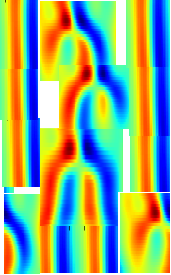
\includegraphics[width=0.25\textheight,height=.36\textheight]{MNG_ppo_frankenstein}
\end{minipage} \quad\quad
\begin{minipage}[height=.80\textheight]{.25\textheight}
\centering      {\footnotesize\texttt{\quad\quad 2-torus}}
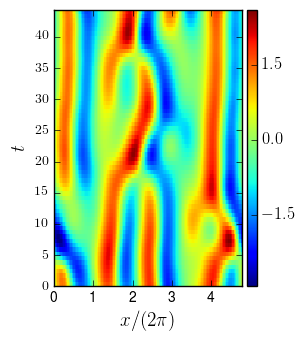
\includegraphics[width=0.35\textheight,height=.45\textheight]{MNG_ppo_L30_T44}
\end{minipage} \qquad\qquad
  \end{block}
\end{frame}

\begin{frame}{turbulence.zip : each solution has a unique symbolic name}
  \begin{block} {symbolic dynamics is 2\dmn!}
  \begin{center}
  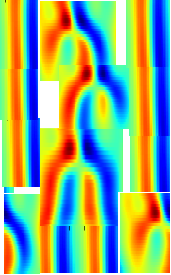
\includegraphics[width=.25\textwidth,height=.4\textheight]{MNG_ppo_frankenstein}
~~~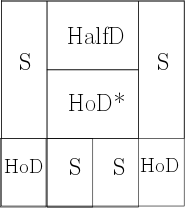
\includegraphics[width=.25\textwidth,height=.4\textheight]{MNG_approxsymbdyn}
~~~\includegraphics[width=.25\textwidth,height=.4\textheight]{MNG_approxsymbdyntrinary}
%  \includegraphics[width=.3\textwidth,height=.3\textheight]{MNG_ppo_L30_T44}
  \end{center}
  \end{block}
\begin{itemize}
 \item each symbol indicates a corresponding spatiotemporal tile
 \item these are ``rubber'' tiles
\end{itemize}
\end{frame}

%%%%%%%%%%%%%%%%%%%%%%%%%%%%%%%%%%%%%%%%%%%%%%%%%%%%%%%%%%%%%%%%
\begin{frame}{part 5}
\begin{enumerate}
              \item
    \textcolor{gray}{\small
turbulence in large domains
              \item
space is time
    }
              \item
    {\Large
bye bye, dynamics
    }
            \end{enumerate}
\end{frame}

\begin{frame}{in future there will be no future}
\begin{center}
{\huge goodbye}
\end{center}

\vfill

to long time and/or space integrators
\medskip

\hfill they never worked and could never work
\end{frame}

\begin{frame}{life outside of time}
\textcolor{red}{the trouble}:

forward time-integration codes too unstable
\bigskip
\bigskip

\textcolor{blue}{multishooting inspiration}:
 replace a guess that a  \textcolor{blue}{point} is on the periodic
orbit by a guess of the \textcolor{blue}{entire orbit}.
\bigskip

$\to$
\bigskip

spatio-temporally periodic solutions of classical field theories
can be found by \textcolor{blue}{variational methods}
\end{frame}

\begin{frame}{can computers}

\vfill

{\Huge
do this ?
                  }
\vfill
\end{frame}

\begin{frame}{the very short answer : POT}
\includegraphics[width=1.0\textwidth]{MvSydow7seal.jpg}
\bigskip
if you win : I teach you how

\vfill\hfill (for details, see \wwwcb{})
\end{frame}

\begin{frame}{the answer is}

\vfill

{\Huge
scalability
                  }

\vfill

%\hfill in the spirit of this workshop
\end{frame}

\begin{frame}{compute locally, adjust globally}
\begin{block}{Navier-Stokes codes}
\begin{itemize}
 \item
T. M. Schneider : developing a matrix-free variational Navier-Stokes code,
machine learning initial guesses
 \item
D. Lasagna and A. Sharma  : developing variational adjoint solvers to
find periodic orbits with long periods
 \item
Q. Wang : parallelizing {\color{red}spatiotemporal}
computation is FLOPs intensive, but more robust than
integration forward in time
\end{itemize}
\end{block}

\vfill\hfill
it's rocket science%
\footfullcite{Schneider19}$^,$%
\footfullcite{LaShMe18}$^,$%
\footfullcite{WGBGQ13}
%\footnote{{\tiny Q. Wang \etal,}\HREF{https://doi.org/10.1063/1.4819390}
%{\tiny\em Towards scalable parallel-in-time turbulent flow simulations},
%{\tiny Physics of Fluids (2013)}}
\end{frame}

\begin{frame}{
towards scalable parallel-in-time turbulent flow simulations
}
\begin{block}{future :}%
processor speed $\to$ limit

\medskip

number of cores $\to 10^6 \to \cdots$

\medskip
\end{block}

\emph{Q. Wang% et al (2013)
    \footfullcite{WGBGQ13}%$^,$\footfullcite{Ihara66}
    :} % Gomez, Blonigan, Gregory and Qian 2013 :}

next-generation simulation paradigm : spacetime parallel
simulations, on discretized $4D$ spacetime
computational domains, with each computing core handling a spacetime lattice cell

\bigskip

compared to time-evolution solvers:
significantly higher level of concurrency, reduction the ratio of
inter-core communication to floating point operations

\bigskip

$\qquad\qquad\Rightarrow$ a path towards exascale DNS of turbulent flows
\end{frame}

\begin{frame}{Dreams of Grand Schemes :  solve}
 \begin{center}
   \includegraphics[width=0.60\textwidth]{02-DreamEqs}
 \end{center}
\end{frame}

\begin{frame}{machine learning will be needed}
``reservoir computing'' example\footfullcite{PHGLO18}

\bigskip

 \begin{columns}
 \column{0.35\textwidth}
~~~~~~\includegraphics[width=1\textwidth]{PHGLO18fig2}
 \column{0.65\textwidth}
 \begin{itemize}
 \item[(a)] data: \\ \KS\ simulation
 \item[(b)] reservoir computing prediction
 \item[(c)] two subtracted agree to \\
            $\sim 5$ Lyapunov times
 \end{itemize}
 \end{columns}
\vfill\hfill\textcolor{red}{\huge how would you learn this data?}
\end{frame}


\begin{frame}{take home : clouds do not solve PDEs}

%and do they care what PST hour is it?
%\\
%and at what longitude are they?
%\\
do clouds integrate Navier-Stokes equations?

\begin{center}
\centerline{\textcolor{red}{\Huge NO!}}
%\end{center}
%for weather prediction, we store sets of weather sequences
%\bigskip\bigskip

%\begin{center}
\begin{minipage}[t]{\textwidth}
	\begin{center}
%\vspace{2ex}
\centerline{
\raisebox{-4.0ex}[5.5ex][4.5ex]
		 {\includegraphics[height=12ex]{Hopf-a}}
~~~ $\Longrightarrow$ ~~ {other swirls} ~~ $\Longrightarrow$ ~~~
	\raisebox{-4.0ex}[5.5ex][4.5ex]
		 {\includegraphics[height=12ex]{Hopf-b}}
          }
	\end{center}
\end{minipage}
\end{center}

at any spacetime point Navier-Stokes equations describe the local tangent space

\bigskip

\centerline{
\textcolor{blue}{they satisfy them \textcolor{red}{\large locally}, everywhere and at all times}
}
\end{frame}


\begin{frame}{summary}
\begin{enumerate}
              \item
study turbulence in infinite spatiatemporal domains
              \item
theory : classify all spatiotemporal tilings
              \item
numerics : future is spatiotemporal
\end{enumerate}

\vfill

there is no more time

\medskip

there is only enumeration of spacetime solutions
\end{frame}

\begin{frame}{spatiotemporally infinite \catlatt}
%\begin{center}
%\hfill\includegraphics[width=0.55\textwidth]{spatiotempCat}
\hfill\includegraphics[width=0.55\textwidth]{DawnBishopCats}
%\end{center}
\end{frame}

%\begin{frame}{XXX}
%\end{frame}

\end{document}
